\chapter{Using Fourier transform phase for the measurement of radial velocity}
\label{\thechapter}
\label{ch:Methods}
\addcontentsline{lof}{chapter}{\protect\numberline{\arabic{chapter}} {\nameref{\thechapter}}}

%----------------------------------------------------------------------------------------

\rule{\textwidth}{1.6pt}
\minitoc
\clearpage

%----------------------------------------------------------------------------------------

%{\em CGT: This needs a bit more helpful an introduction. That is WHY the fourier trasform is being explored as
%a way to measure radial velocity. and specifically, so that you can try to tell the difference between bulk line shifts, and line profile deformations.
%I think the folloing does a slightly better job of that.}

This chapter introduces a new method for measuring radial velocities. Specifically, it uses the Fourier transform
of a line profile (or cross-correlation profile) to try and distinguish between the effects of a bulk shift in that profile
(i.e. a radial velocity shift of the profile), opposed to a change in the line profile shape which can produce an
apparent radial velocity shift. We examine the impact on the Fourier transformed components of a line profile of both bulk line shifts, and line profile deformations, with the aim of developing tools to distinguish between these two cases.

%%----------------------------------------------------------------------------------------	
%\pagebreak
%%----------------------------------------------------------------------------------------	

\section{Phase analysis of Fourier transform for the measurement of line shift}
\label{\thesection}
\label{ch:FT_line_shift}

The translation of a function (in our case a spectral line profile) can be examined in both its original real
space, and in its Fourier transformed space. Because Fourier techniques are often used to handle time domain data,
this shift in real space can be variously described as either time shifting or translation. In this chapter 
we will use ``time shifting'', ``translation'' and ``velocity shifting'' interchangeably to refer to a shift of a function
in real space. We will refer to Fourier transformed functions as being in the ``frequency domain'' regardless of whether they have actual dimensions of 1/time, 1/length or 1/velocity.

\subsection{Translation property of Fourier transform}

Let us consider a function $h(x)$ be a signal $f(x)$ delayed (or shifted) by an amount $x_0$:
\begin{equation}
	h(x) = f(x-x_0).
\label{eq:FT1}
\end{equation}
In the frequency domain, we will then have 
\begin{equation}
	\hat{h}(\xi) = e^{-2 \pi ix_0 \xi} \hat{f}(\xi),
\label{eq:FT2}
\end{equation}
where the circumflex denotes the Fourier transform of a function, e.g.
\begin{equation}
	\hat{f}(\xi) = \int_{-\infty}^{\infty} f(x) e^{-2 \pi ix \xi} dx.
\label{eq:FT3}
\end{equation}
This is saying (E.q.~\ref{eq:FT2}), $\hat{h}(\xi)$ and $\hat{f}(\xi)$ differ by a frequency dependent phase angle: 
\begin{equation}
	\Delta \phi(\xi) = -2 \pi x_0 \xi,
\label{eq:PhaseShift}
\end{equation}
while the power spectral density will remain unchanged, i.e. $\mid \hat{h}(\xi)\mid ^2 = \mid\hat{f}(\xi)\mid^2$ as $\mid e^{-2 \pi ix_0 \xi}\mid ^2 = 1$.

\subsection{Intuitive explanation}

The translation property of the Fourier transform can be derived easily by the interested reader. A (perhaps) more intuitive but equally quantitative way to see this is as follows: the Fourier transform decomposes the function $f(x)$ into a frequency representation $\hat{f}(\xi)$, each frequency component accompanied by the orthogonal basis $e^{2 \pi ix \xi}$, as in the form of inverse Fourier transform: 
\begin{equation}
	f(x) = \int_{-\infty}^{\infty} \hat{f}(\xi) e^{2 \pi ix \xi} d\xi. 
\end{equation}
Shifting $f(x)$ by $x_0$ in the time domain is equivalent to shifting \textit{all} the orthogonal basis functions by $x_0$, which becomes $e^{2 \pi i(x-x_0) \xi} = e^{2 \pi i x \xi} \cdot e^{-2 \pi ix_0 \xi}$. This is how the $e^{-2 \pi ix_0 \xi}$ term in Eq.~\ref{eq:FT2} arises -- it quantifies the phase difference. 

A (probably) even more intuitive but less quantitative way to vision the relation between a shift of the signal and a phase difference is to imagine any real continuous function is a sum of sines and cosines. Changing the phase angle in the sines and cosines results in shifts in the function. 

Moreover, the fact that the power spectrum density remains the same is because shifting the signal as a whole doesn't add or remove any frequency components. 


\subsection{Practical Use}

From Eq.~\ref{eq:PhaseShift}, we see that the phase shift $\Delta \phi(\xi)$ is proportional to the frequency $\xi$ with a constant gradient or slope
\begin{equation}
	\dv{(\Delta \phi)}{\xi} = -2 \pi x_0
\label{eq:gradient}
\end{equation}
where we use $\Delta$ to refer to the phase difference between a shifted line profile and a unshifted~/~referenced line profile, while the derivative to refer to the response of $\Delta \phi$ to $\xi$. $\phi(\xi)$ can be obtained by extracting the phase information from the Fourier transform of line profiles. After that, a simple linear regression model fit to a plot of $\Delta \phi(\xi)$ versus $\xi$ (Fig.~\ref{fig:FT}) will enable us to measure the bulk shift between two line profiles $x_0$. 

%-------------
\begin{figure}[tbp]
\centering
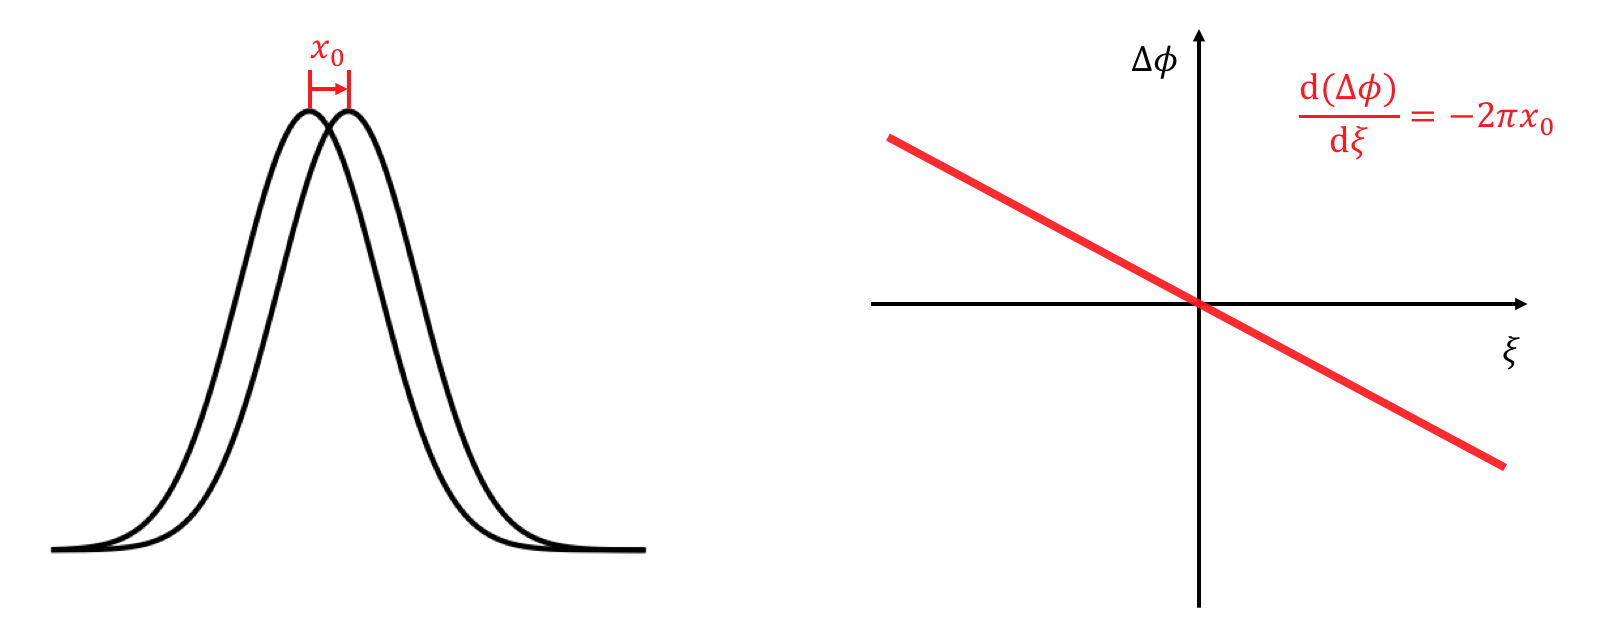
\includegraphics[width = 0.99 \linewidth]
{./Figures/Methods/FT.png}
\caption[Translation property of Fourier transform]
{The left panel shows a signal (or a spectral line profile in the following context) shifted by an amount $x_0$. 
The right panel is the differential phase spectral density diagram (i.e. differential phase spectrum). 
The model shows the phase difference between two shifted signals $\Delta \phi(\xi)$ and the frequency $\xi$ are linearly correlated. Its slope $-2 \pi x_0$ contains information of the amount of signal shift in time domain.}
\label{fig:FT}
\end{figure} 
%-------------

By analogy with the definition of power spectral density or power spectrum, we describe $\phi(\xi)$ the \textbf{phase spectral density} or \textbf{phase spectrum} and hence $\Delta \phi(\xi)$ the \textbf{differential phase spectral density} or \textbf{differential phase spectrum}. In this approach, an analysis of the phase shift in the frequency domain of the Fourier components of a line profile will provide a means of measuring a bulk line shift in real space. We therefore name our method \textbf{Fourier phase spectrum analysis}. 
% More importantly,
% it may provide a means of separating  an apparent radial velocity shift into the components due to bulk line shift, 
% and line profile shape change.


%----------------------------------------------------------------------------------------	

\subsection{Initial tests}
\label{sec:Initial_tests}

We performed an initial test to determine that we can correctly recover known shifts of a line profile using the Fourier phase spectrum analysis. We generated a spectral line profile based on the cross-correlation function of observed HARPS spectra with the software SOAP 2.0 \cite{Dumusque2014SOAP}. This was replicated 100 times, with a very small amount of 
noise (equivalent to a S/N = 10,000) injected in each of the line profiles. These profiles were then
subjected to radial velocity shifts evenly spaced between 0 and 10\,m/s (Fig.~\ref{fig:line_profiles12}). 

%-------------
\begin{figure}[tbp]
    \begin{subfigure}[b]{0.49\textwidth}
        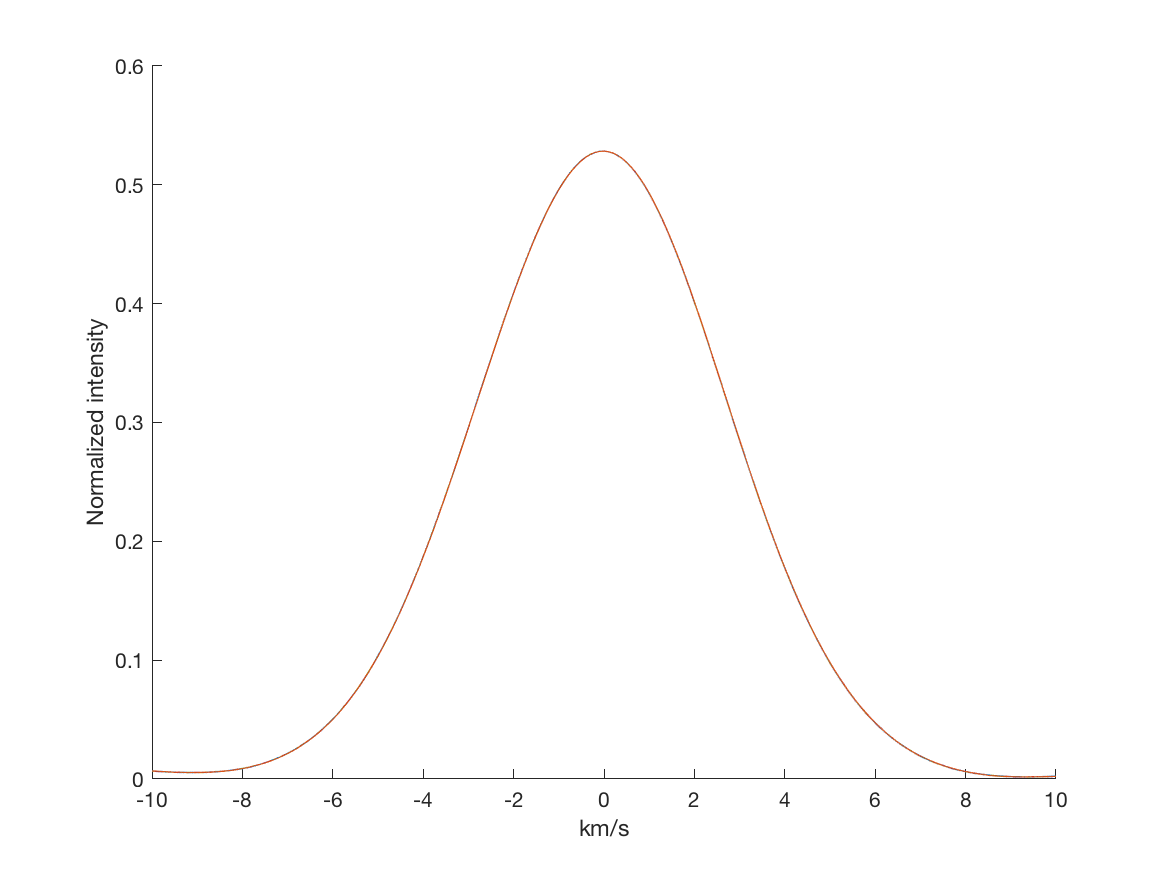
\includegraphics[width=\textwidth]{./Figures/Methods/1-Line_Profile.png}
        \caption{Line profile (stacked)}
        \label{fig:line_profiles}
    \end{subfigure}
	~
    \begin{subfigure}[b]{0.49\textwidth}
        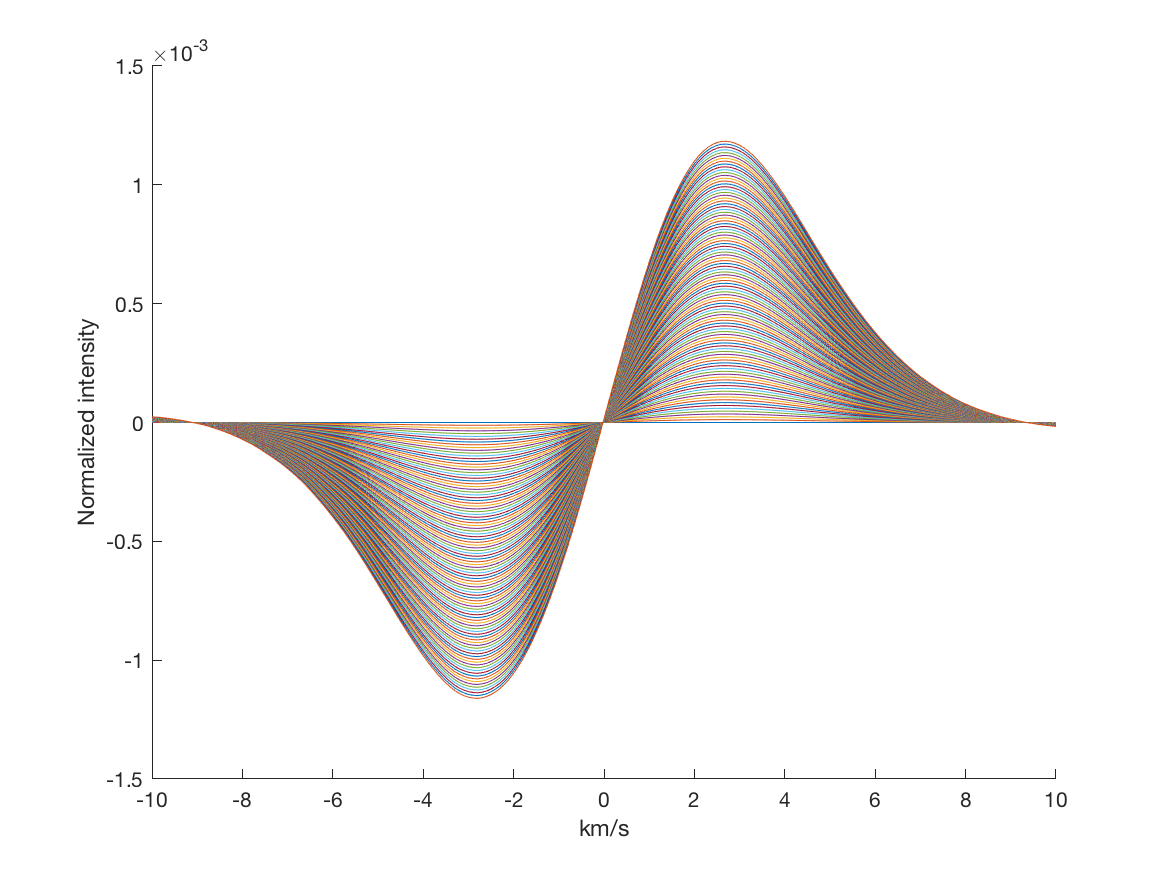
\includegraphics[width=\textwidth]{./Figures/Methods/1-Differential_line_Profile.png}
        \caption{Differential line profile}
        \label{fig:differential_line_profiles}
    \end{subfigure}	
    
    \caption[100 shifted HARPS-like line profiles]{(a) the shifted line profiles plotted on top of each other, showing that the 0-10\,m/s shifts are very small compared to the line profile width. (b) the shifted line profiles with the unshifted line profile subtracted from each. Note that for the sake of clarity, the differential line profiles are plotted noise-free and only 10 out of 100 profiles are presented.}
\label{fig:line_profiles12}
\end{figure}	
%-------------

The Fourier transform of these 100 spectral line profiles divides the information into two parts: (1) the power spectra (Fig.~\ref{fig:power_spectrum}) and (2) the phase spectra (shown in Fig.~\ref{fig:dps} as the differential phase spectra relative to the phase spectrum of the unshifted line profile). We see that most information is concentrated towards the centre of the power spectrum (i.e. the lower frequency range), and as expected, the differential phase spectra are mostly linear (consistent with the theory demonstrated in Fig.~\ref{fig:FT}). Its deviation from linearity comes from the noise that we injected, which will be discussed later. 

%-------------
\begin{figure}[tbp]	
    \begin{subfigure}[b]{0.49\textwidth}
        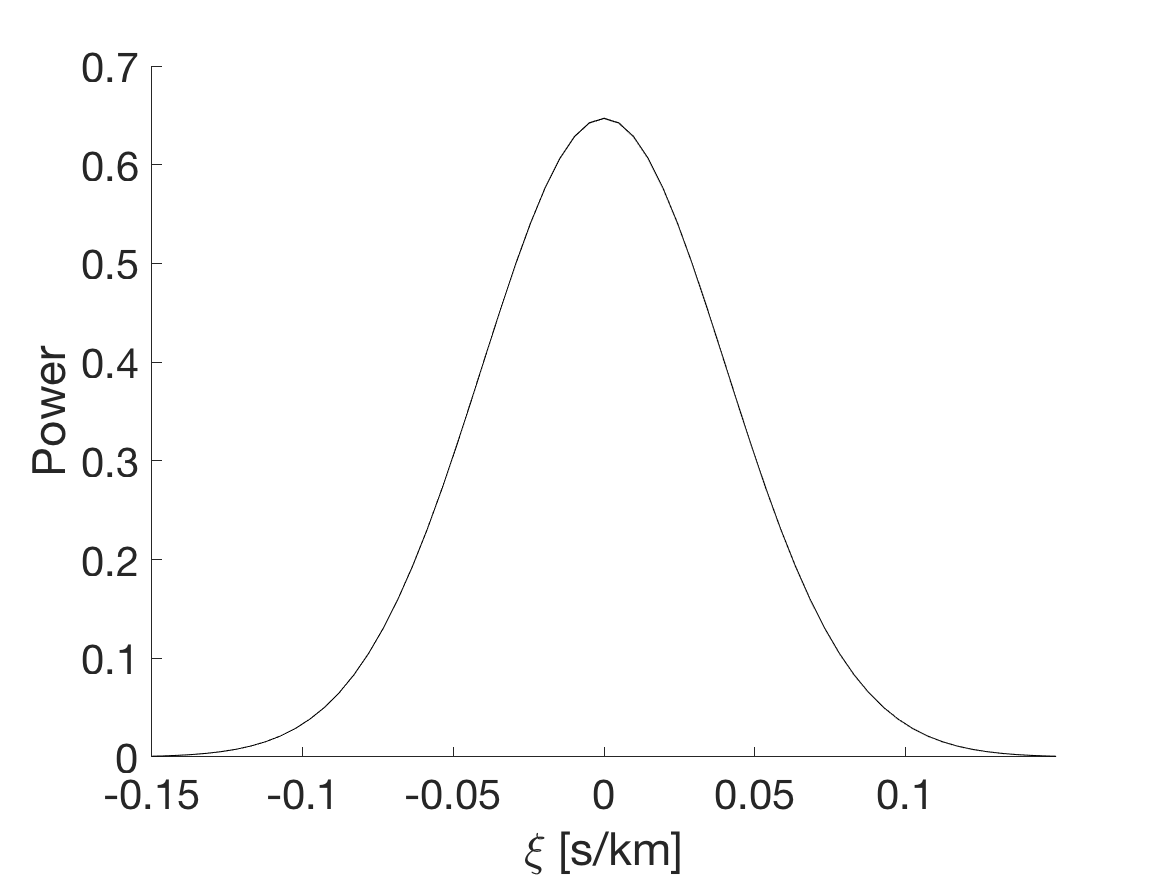
\includegraphics[width=\textwidth]{./Figures/Methods/2-FT_power.png}
        \caption{Power spectrum (stacked)}
        \label{fig:power_spectrum}
    \end{subfigure}
	~
    \begin{subfigure}[b]{0.49\textwidth}
        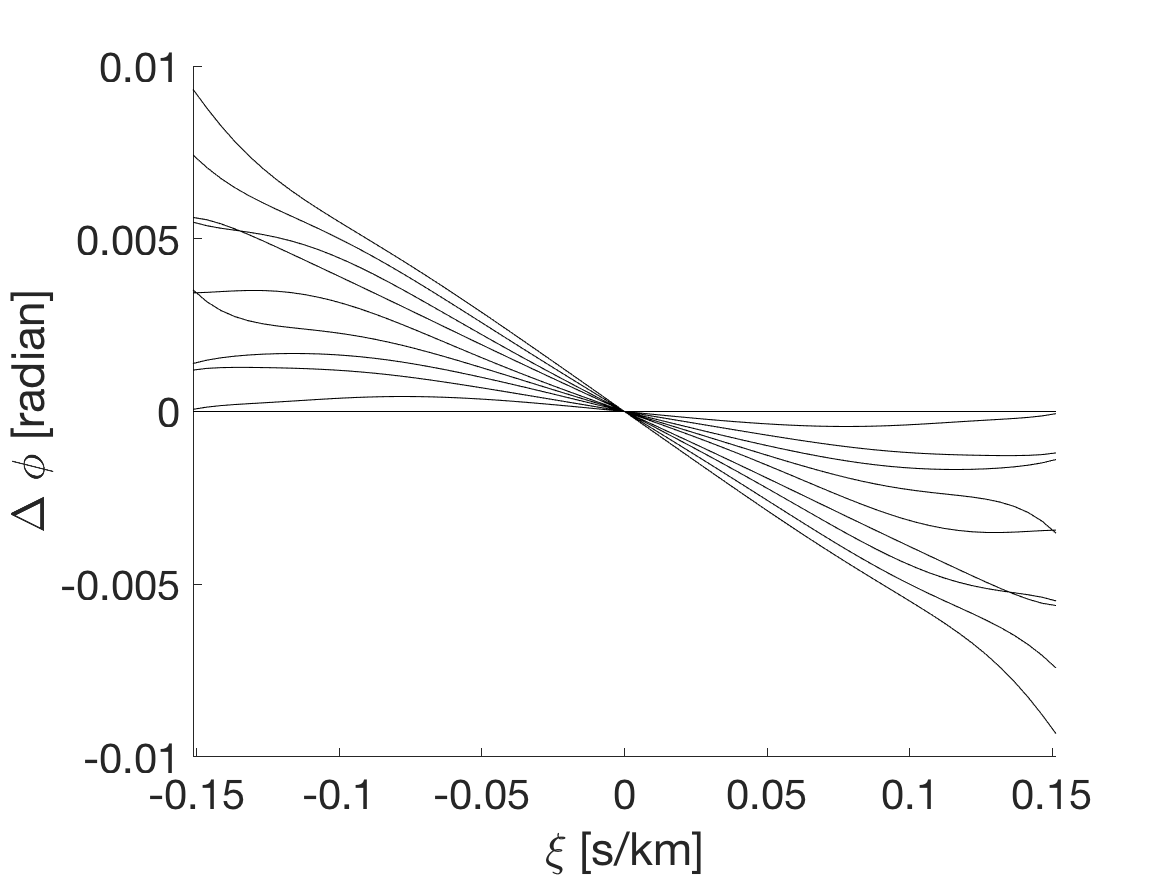
\includegraphics[width=\textwidth]{./Figures/Methods/4-Relative_phase_angle.png}
        \caption{Differential phase spectrum}
        \label{fig:dps}
    \end{subfigure}	
    \caption[Fourier transform of 100 shifted line profiles]
    {The Fourier transform of these shifted line profile divides the information in each into (a) their power spectra and (b) their phase spectra (here plotted differential compared to that of the unshifted profile). A line shift in the time domain produces an unchanged power spectrum in the frequency domain. It does, however, produce phase shifts which we see as linear trends in the differential phase spectra as a function of frequency. Note that for demonstration clarity, only 10 out of 100 differential phase spectra are presented.}
\label{fig:FT_process}
\end{figure}    
%-------------

The slope of each differential phase spectrum indicates the shift of each line profile relative to the unshifted one. For a linear regression fitting, each frequency sample on the differential phase spectrum is weighted by the amplitude of the power, meaning the lower frequencies are more weighted. We calculate the radial velocity shift for each shifted line profile using two methods: (1) Fourier phase spectrum analysis that delivers $RV_\text{FT}$; (2) traditionally measuring the line centroid by fitting a Gaussian function to each line profile that delivers $RV_\text{Gaussian}$. 

We then compare the both $RV_\text{FT}$ and $RV_\text{Gaussian}$ with the known input line shift. Fig.~\ref{fig:rv_recovery} sees the expected strong 1:1 correlation between the input radial velocity shift and the output -- the line of best fit of a linear regression model presents a slope of $1.003\pm0.006$ with 95\% confidence bounds for both $RV_\text{FT}$ and $RV_\text{Gaussian}$. 
% The uncertainty of the slope is derived from the uncertainty of each measured $RV_\text{FT}$, which is further derived from the uncertainty of the phase measurement, described by the magnitude of the power spectrum.
The root-mean-square (rms) of the residuals (or interchangeably used as standard deviation when the mean is zero) are both $\sigma_\text{FT} = \sigma_\text{Gaussian} = 0.08$ m/s, identical up to two decimal places, indicating the expected radial velocities are consistently obtained using both methods. In fact, the almost overlapping residual in Fig.~\ref{fig:rv_recovery} meaning that the two methods are so coherently different from the input radial velocity (by a small amount), leads us to conclude that such a deviation comes from the photon noise intrinsic to the line profile rather than the methods themselves. 

%-------------
\begin{figure}[tbp]
\centering
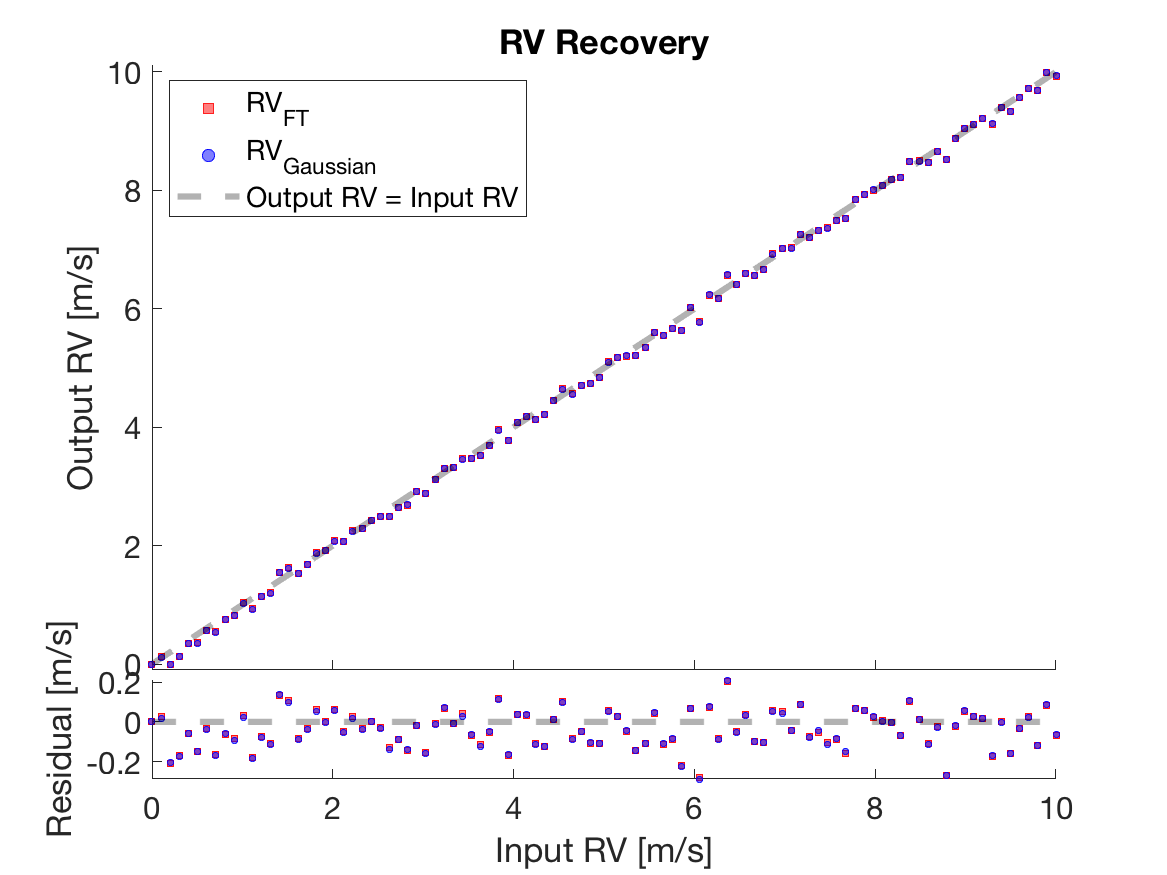
\includegraphics[width = 0.7 \linewidth]
{./Figures/Methods/5-LINE_SHIFT_ONLY.png}
\caption[Radial velocity recovery]
{Radial velocity recovery of line shifts with both methods: Fourier transform and Gaussian fit. Both results are highly consistent with each other. Errorbars are not plotted for clarity.}
\label{fig:rv_recovery}
\end{figure} 
%-------------
\FloatBarrier

{\em CGT: How do these comare which what you'd expect from the S/N and the intrinsic line width (should say at some int what the intrinsic line width is}.


%----------------------------------------------------------------------------------------	

\subsection{Further tests}
\label{sec:Further_tests}

Let's recall the justification of measuring a line shift in its Fourier space -- the shifting of a line (or a function), when viewed as shifting the sum of its Fourier basis functions (or any other basis functions), has equally the same amount of shift on every basis function, which can be measured as a phase shift in the Fourier phase spectrum. That is to say, utilising only part of the phase spectrum will also return the correct amount of shift of a line profile, although it is more likely to be affected by noise. The motivation of this practice will be discussed in \S\ref{sec:FT_ld} when it comes to line profile deformations, whereas we simply lay out the tests in this subsection. 

We choose to divide the whole frequency range into two parts (Fig.~\ref{fig:low-high-pass}) -- the lower frequency range (i.e. apply a low-pass filter) and the higher frequency range (i.e. apply a high-pass filter). The dividing frequency $\xi_{HL}$ is chosen such that both the lower and higher frequency ranges take up half of the power spectrum $P(\xi)$:
\begin{equation}
	\int_{\xi_{L}=0}^{\xi_{HL}} P(\xi) d\xi = \int_{\xi_{HL}}^{\xi_{H}} P(\xi) d\xi. 
\end{equation}
We assume the integration of power spectrum is a measurement of the amount of ``information", so that in a noise-free circumstance, we would put equal trust on the radial velocities obtained from the lower and higher frequencies (namely $RV_\text{FT,L}$ and $RV_\text{FT,H}$, or $RV_\text{FT,H/L}$ for both), though this does not necessarily deliver equal credibility between them in practice. In addition, a cut-off frequency $\xi_{H}$ applies to the upper boundary of the high-pass filter. Frequencies higher than $\xi_{H}$ hardly contributes to the shape of the line profile as $P(\xi)$ converges to zero, and they can be impacted by noise in a unpredictable way. $\xi_{H}$ is chosen empirically where $P(\xi)$ drops to $0.1\%$ of the highest $P(\xi)$.

%-------------
\begin{figure}[tbp]	
    \begin{subfigure}[b]{0.49\textwidth}
        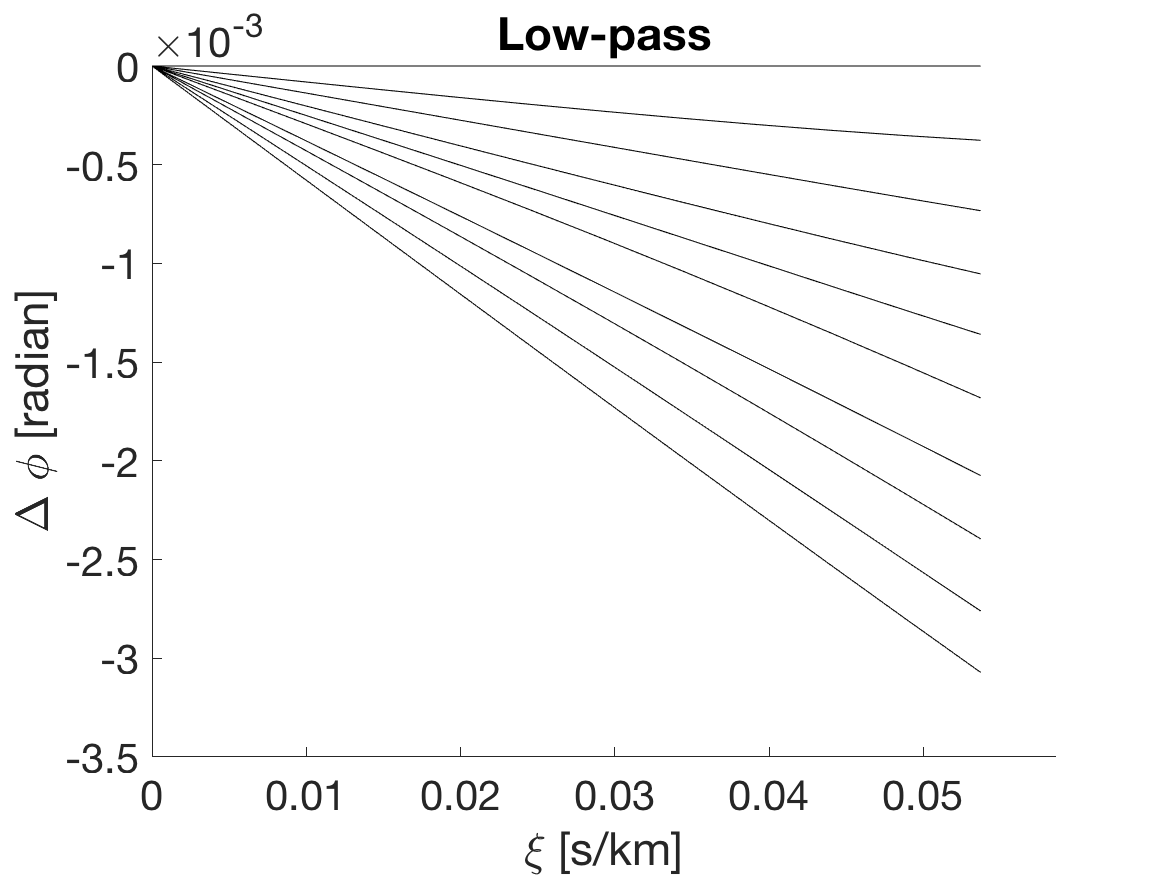
\includegraphics[width=\textwidth]{./Figures/Methods/4-Relative_phase_angle_L.png}
    \end{subfigure}
	~
    \begin{subfigure}[b]{0.49\textwidth}
        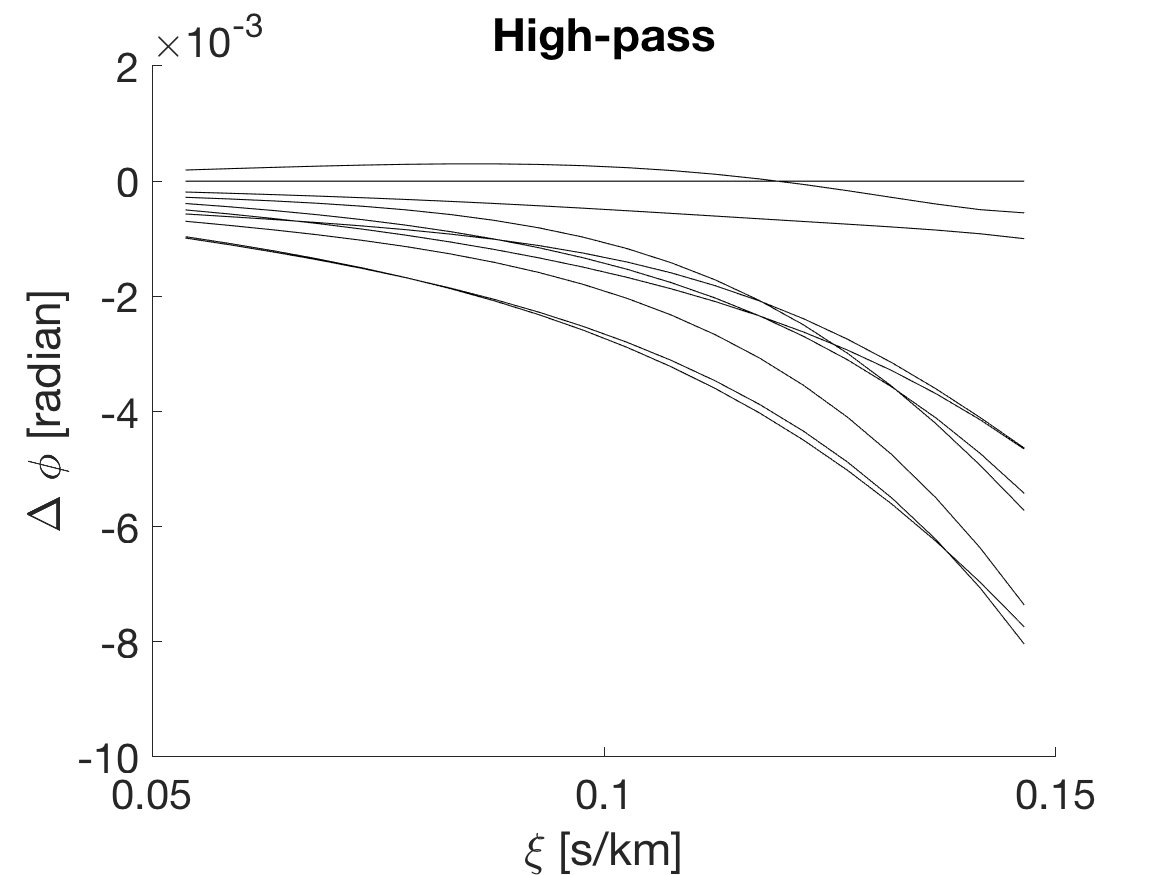
\includegraphics[width=\textwidth]{./Figures/Methods/4-Relative_phase_angle_H.png}
    \end{subfigure}	

    \caption[Low-pass and high-pass filters]
    {Differential phase spectrum as shown in Fig.~\ref{fig:dps} sub-divided into lower frequency range and higher frequency range. Only the non-negative ranges are plotted.}
\label{fig:low-high-pass}
\end{figure}    

Fig.~\ref{fig:rv_recovery} presented an accurate recovery of the radial velocity shift given by $RV_\text{FT}$, for which we made use of the full range of frequencies; in Fig.~\ref{fig:rv_recovery_LH}, it still manages to deliver a good 1:1 alignment between $RV_\text{FT,H/L}$ and the input radial velocity. The line of best fit presents a slope of $1.002\pm0.007$ for $RV_\text{FT,L}$ and $0.977\pm0.029$ for $RV_\text{FT,H}$ respectively, with 95\% confidence bounds. The scatter of the residuals are $\sigma_\text{FT,L} = 0.11$ m/s and $\sigma_\text{FT,H} = 0.43$ m/s. Firstly, we note that $\sigma_\text{FT,H/L} > \sigma_\text{FT}$, this is because both $RV_\text{FT,H}$ and $RV_\text{FT,L}$ scarify part of frequency information in the Fourier space for the different response to line deformation. Secondly, we note that $RV_\text{FT,H} > RV_\text{FT,L}$, seemingly contradicting with the expectation that equal amount of ``information" from which they are derived should deliver the equivalent amount of scatter in the residuals. We think this may be because higher frequency modes are more likely to be subjected to stochastic behaviours other than the line deformation arising from stellar variability generated in the SOAP model. For example, the fluctuations of photon levels on the stellar spectrum are mainly described by high frequency modes. {\em jzhao: Have I made myself clear here?}

%-------------
\begin{figure}[tbp]
\centering
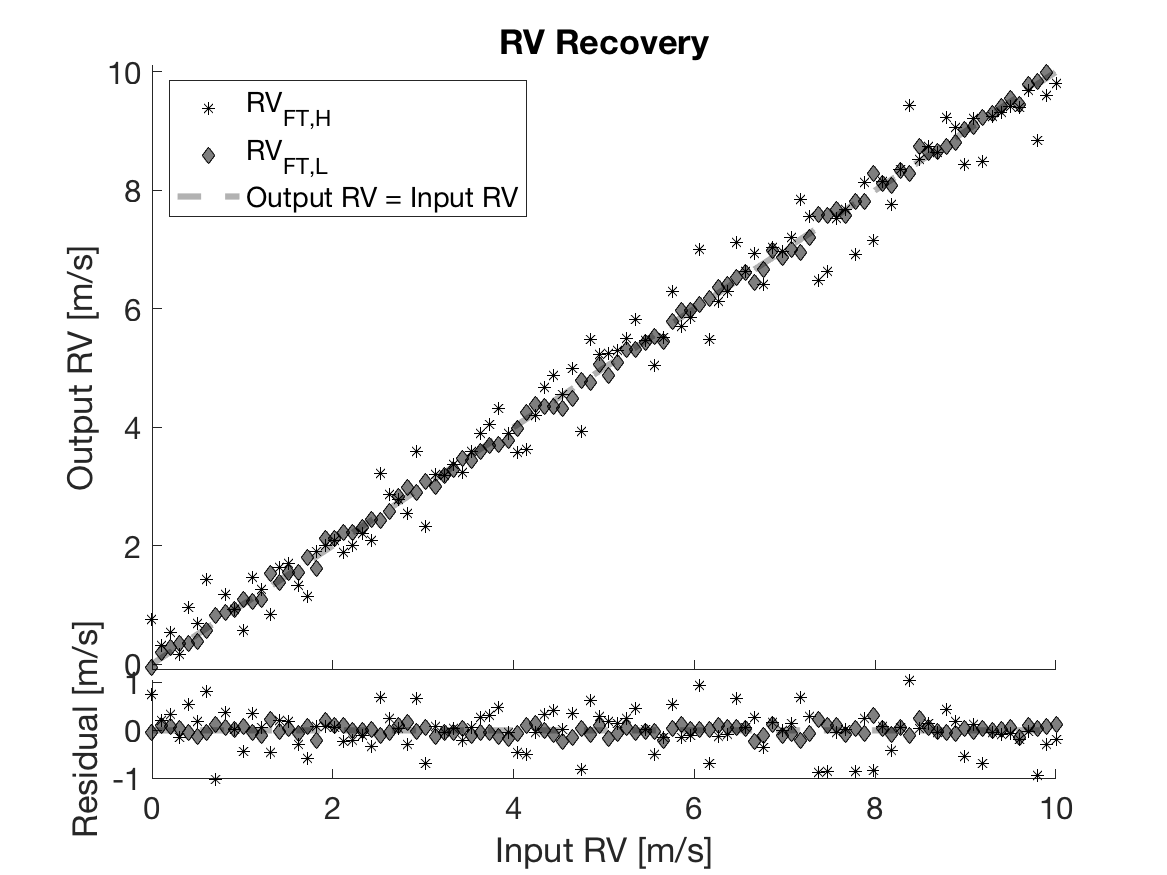
\includegraphics[width = 0.7 \linewidth]
{./Figures/Methods/5-LINE_SHIFT_ONLY-HL.png}
\caption[Low-pass and high-pass radial velocities]
{Radial velocity recovery of line shifts with low-pass and high-pass filters. Errorbars are not plotted for clarity.}
\label{fig:rv_recovery_LH}
\end{figure} 
%-------------
\FloatBarrier

%----------------------------------------------------------------------------------------
\subsection{Cut-off frequency}
\label{sec:noise}

We briefly mentioned in \S\ref{sec:Initial_tests} that the deviation from linearity in the differential phase spectrum arises from the photon noise injected in the simulated line profiles, and in \S\ref{sec:Further_tests} that introducing a cut-off frequency in the upper boundary avoids dealing with excessive noise. This can be visually explained with the Fourier transformed line profile $\hat{h}(\xi)$ in a complex plane (also known as the Argand plane; Fig.~\ref{fig:FT_compelx_plane}). What we see is $\hat{h}(\xi)$ literally plotted on the complex plane, for the frequencies that are sampled. Of each complex number $\hat{h}(\xi)$, the argument returns the phase angle and the square of the absolute value returns the power. For larger powers (i.e. $\hat{h}(\xi)$ far from the origin as viewed in Fig.~\ref{fig:FT_compelx_plane} left), the presence of noise (S/N = 10,000) hardly alters the phase angle; for lower powers (i.e. $\hat{h}(\xi)$ distributed in the vicinity of the origin as viewed in Fig.~\ref{fig:FT_compelx_plane} right), a slight displacement of $\hat{h}(\xi)$ in the complex plane means a considerable change in the phase angle in the presence of even a tiniest amount of noise (S/N = 10,000). It justifies using the Fourier transform spectral power to be the weight of each frequency, and introducing a cut-off frequency when making a linear fit of the differential phase spectrum. 

Another possible reason to introduce the cut-off frequency is the periodicity of the basis functions in a Fourier transform. The basis function $e^{-2 \pi ix_0 \xi}$ repeats itself at the period of $1/\xi$, making measuring the shift in the time domain larger than the order of $1/\xi$ degenerate (i.e. the shifts of $x_0+k/\xi$ for $k\in\mathbb{Z}$ become indistinguishable). Nevertheless, this is very unlikely the case that we may encounter. In the test examples above, the cut-off frequency is $\xi = 0.15$ s/km, corresponding to the period of $1/\xi\sim6.7$ km/s, which is way larger than the radial velocities induced by planets that we normally study at scales of m/s amplitudes. 

%-------------
\begin{figure}[tbp]	
    \begin{subfigure}[b]{0.49\textwidth}
        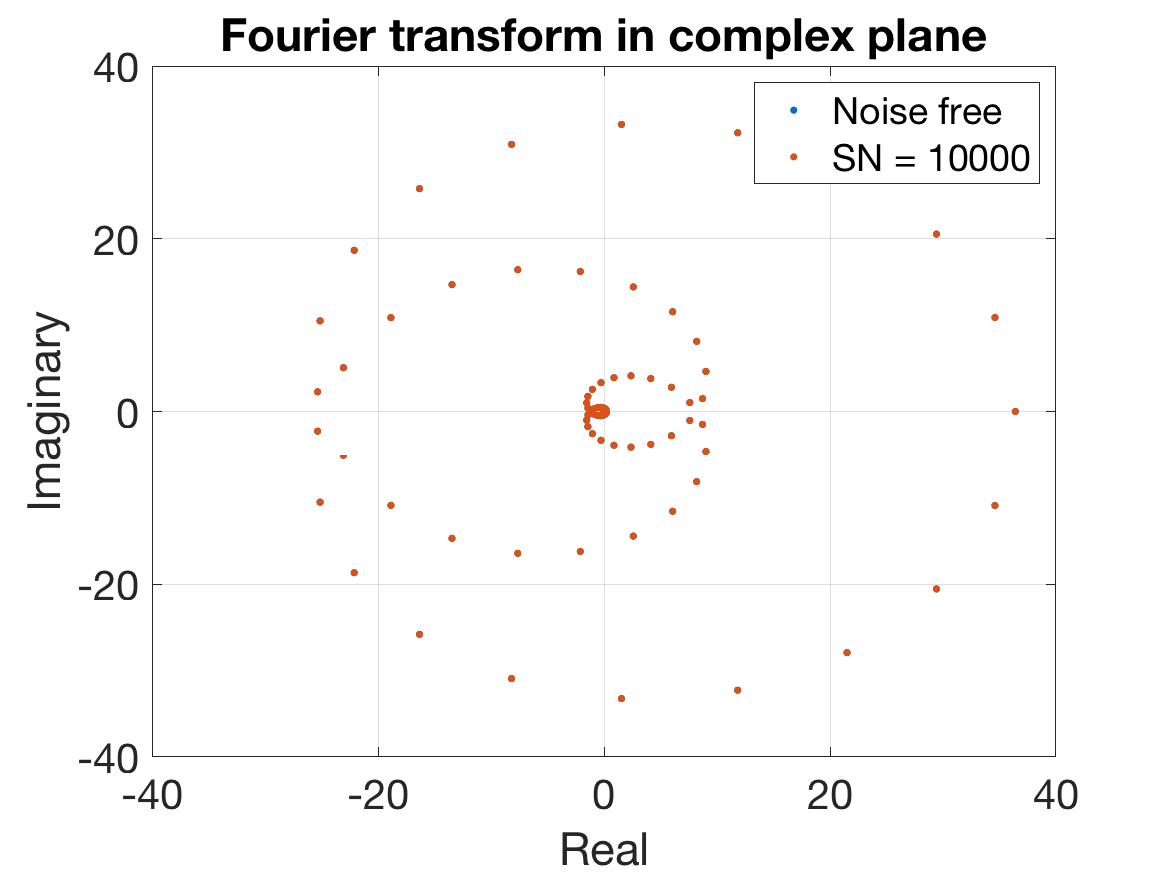
\includegraphics[width=\textwidth]{./Figures/Methods/7-Phase_angle_in_complex_plane_1.png}
%        \caption{Power spectrum (stacked)}
        \label{fig:FT_compelx_plane_1}
    \end{subfigure}
	~
    \begin{subfigure}[b]{0.49\textwidth}
        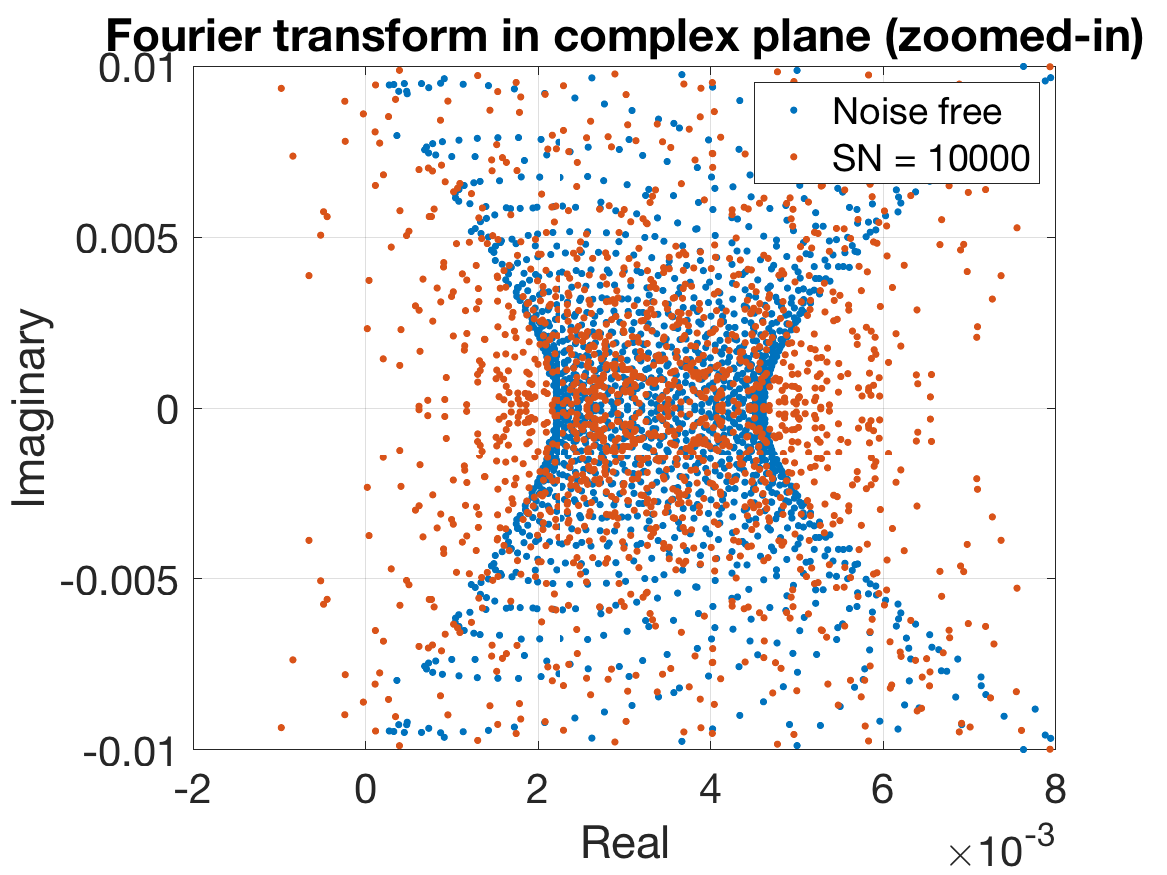
\includegraphics[width=\textwidth]{./Figures/Methods/7-Phase_angle_in_complex_plane_2.png}
%        \caption{Differential phase spectrum}
        \label{fig:FT_compelx_plane_2}
    \end{subfigure}	
    
    \caption[Fourier transform of a line profile in a complex plane]
    {The Fourier transform of a line profile in a complex plane. The right figure is a zoom-in of the left near the origin.}
\label{fig:FT_compelx_plane}
\end{figure}    
%-------------
\FloatBarrier

%This is because we only use part of the information from the original line profile -- both because we utilise a limited range of the differential phase spectra, and because we use only the phase spectra to measure this shift (ignoring the power spectra), while the total information in the original shifted line profile is contained in the combination of the power and phase spectra. 
%
%{\em CGT: This needs more work. You need to show the region you are not using to explain why you choose a more linited range, and
%then say why you chose that more limited range and justify it. Don't just say "higher frequency}.
%
%In fact, higher frequency range becomes useless 
%as the interpretation of Fourier transform in high frequencies is dominated by noise and does not represent the 
%intrinsic shift of the line profile any more. As a result, linearity of phase spectrum breaks down in higher frequencies. 
%The range of ``useful" frequencies will depend on the amount of noise (i.e. S/N). 

%----------------------------------------------------------------------------------------	

\subsection{Conclusion}
In this section, we have introduced a new method for measuring radial velocities -- Fourier phase spectrum analysis. The tests that we have made based on shifting a simulated line profile confirm our proposal that using the differential Fourier phase spectrum, it is possible to measure a radial velocity to similarly high precision. This provides an alternative to the traditional means of obtaining the radial velocities via centroiding the line profile in real space. 

In a broader context, this method will be applicable to measuring shifts of any pattern, and can be extended to higher dimensions. In this thesis, we primarily focus on its use to measure radial velocity shifts in spectral line profiles, and especially whether the Fourier transform phase velocity is more robust against the influence of changes in line deformation than traditional techniques.

\pagebreak
%----------------------------------------------------------------------------------------	
%----------------------------------------------------------------------------------------	

\section{Using the Fourier transform to probe line deformation}
\label{\thesection}
\label{sec:FT_ld}

In \S~\ref{ch:FT_line_shift}, we have tested that the Fourier phase spectrum analysis correctly measures the actual line profile shifts due to a bulk motion of the emitting star. In this section, we wish to test whether this method is more robust against spurious apparent radial velocity shifts produced by changes in the line profile shape in an emitting stars.

%----------------------------------------------------------------------------------------	

\subsection{Theory}
\label{sec:LD_Theory}

For a shift of a line profile by a small amount $x_0$, the same shift $x_0$ applies to \textit{all} of its basis functions. As for line deformation due to stellar variability, $x_0$ becomes frequency dependent (here we exclude the case where the result of a line deformation is exactly the same as a line shift, as this becomes indistinguishable by any means of studying the shape of the line profile alone). That is to say, basis functions at different frequencies would be shifted by different amounts, resulting in shape changes (e.g. skewness) in the line profile. Therefore we modify the translation property of Fourier transform by rewriting $x_0$ as $x_0(\xi)$ in Eq.~\ref{eq:PhaseShift}:
\begin{equation}
	\Delta \phi(\xi) = -2 \pi x_0(\xi) \xi.
\label{eq:PhaseShift2_LPD}
\end{equation}
As a result, the local gradient of the differential phase spectrum, instead of $-2 \pi x_0$ in the case of no line profile deformation, becomes 
\begin{equation}
	\dv{(\Delta \phi)}{\xi} = -2 \pi (x_0 + \dv{x_0}{\xi}).
\label{eq:PhaseShift3_LPD}
\end{equation}
Note that the dependency of $\xi$ has been taken out of $\Delta \phi(\xi)$ and 
$x_0(\xi)$ in writing the differential equation above. 

In principle, we could numerically solve the differential equation (either Eq.~\ref{eq:PhaseShift2_LPD} or Eq.~\ref{eq:PhaseShift3_LPD}) based on the measured $\Delta \phi$ or local gradient d$(\Delta \phi)$/d$\xi$ to obtain $x_0(\xi)$, to further seek to understand which frequency modes are more related to stellar variability, on top of all frequency modes respond to a bulk shift of a line profile in the same way. As a simplistic approach, we could use an \textit{averaged} shift $\overline{x_0(\xi)}$ to describe an overall amount of shift of various frequency modes and rewrite Eq.~\ref{eq:PhaseShift2_LPD} as 
\begin{equation}
	\Delta \phi(\xi) = -2 \pi \overline{x_0(\xi)} \xi
\end{equation}
where $\overline{x_0(\xi)}$ is treated as a constant for the range of frequencies that we study. For example, we can divide the frequency range into two to study the effective line shifts in the lower frequency range vs the higher frequency range (i.e. applying a low-pass and a high-pass filter). 

%----------------------------------------------------------------------------------------	

\subsection{SOAP simulations}
\label{sec:Simulations}

In \S~\ref{ch:FT_line_shift}, we had used the SOAP simulator only to generate a line profile that resembles the HARPS observation. In this section, we would use the simulator SOAP~2.0 to study line deformations arising from starspots. 

Without loss of generality, we injected three spots with different longitudes, latitudes and sizes (parameters specified in Table~\ref{table:spot_configurations}) to model an emitting star, and generated 100 cross-correlation functions for the resulting  deformed line profiles evenly sampled throughout the rotation period of the star (Fig.~\ref{fig:line_profiles_deformation}). A very small amount of noise (equivalent to a S/N = 10,000) was also added into the line profiles in the simulation. 

%-------------
\begin{table}[htbp]
\centering
\begin{tabular}{|c|c|c|c|}
\hline 
 & Longitude & Latitude & Size in disk area percentage\\ 
\hline 
Spot 1 & $174^\circ$ & -$14^\circ$ & 0.18\% \\ 
\hline 
Spot 2 & $288^\circ$ & $74^\circ$  & 0.40\% \\ 
\hline 
Spot 3 & $51^\circ$  & $52^\circ$  & 0.50\% \\ 
\hline 
\end{tabular} 
\caption{Spot configurations}
\label{table:spot_configurations}
\end{table}
%-------------

%-------------
\begin{figure}[tbp]
    \begin{subfigure}[b]{0.49\textwidth}
        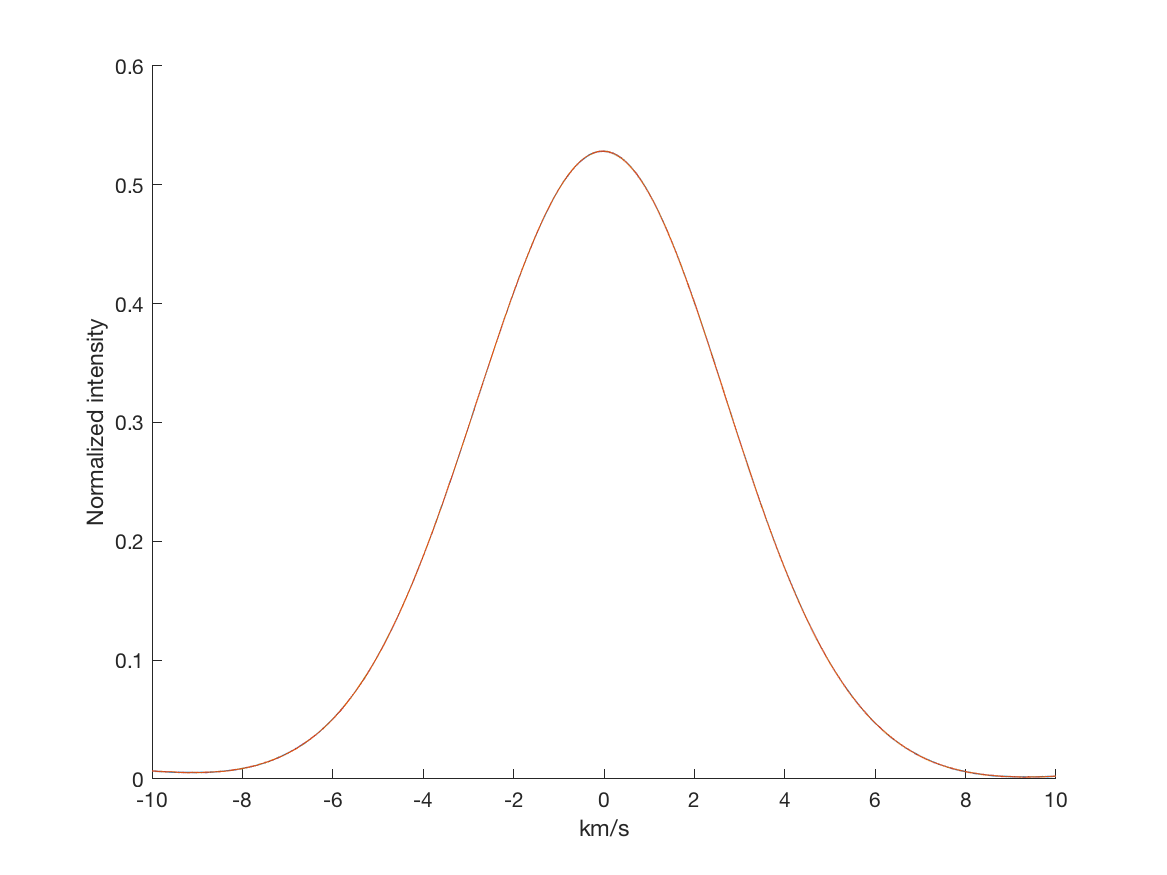
\includegraphics[width=\textwidth]{./Figures/Methods/LPD1-Line_Profile.png}
        \caption{Line profile (stacked)}
    \end{subfigure}
	~
    \begin{subfigure}[b]{0.49\textwidth}
        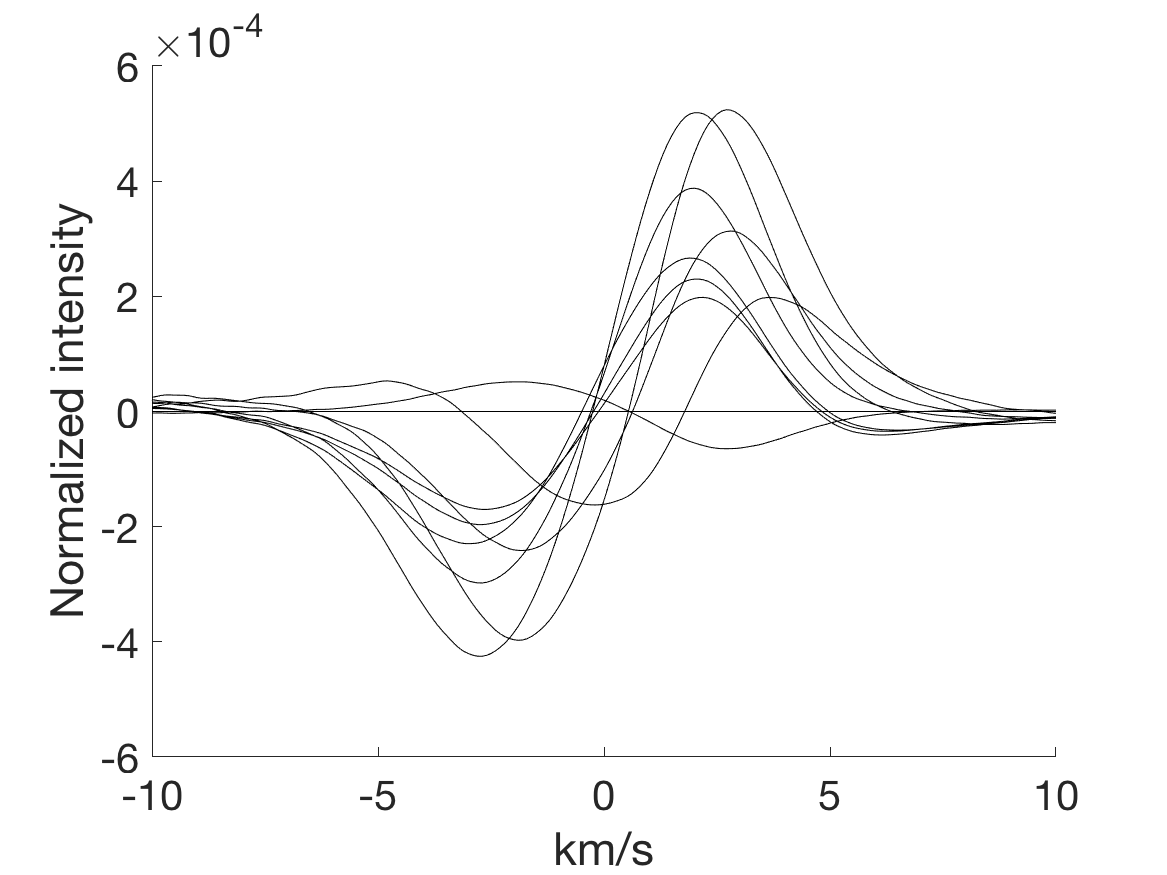
\includegraphics[width=\textwidth]{./Figures/Methods/LPD1-Differential_line_Profile.png}
        \caption{Differential line profile}
        \label{fig:ld_dlp}
    \end{subfigure}	
    
    \caption[Deformed line profile]{Deformed line profile. For the sake of clarity, the differential line profiles are plotted noise-free and only 10 out of 100 profiles are presented.}
\label{fig:line_profiles_deformation}
\end{figure}	
%-------------
\FloatBarrier

%----------------------------------------------------------------------------------------	
\subsection{Fourier phase spectrum analysis}

\subsubsection{$RV_\text{FT}$}
We then take the same approach as in  \S~\ref{ch:FT_line_shift} to obtain the power spectrum and the differential phase spectrum (Fig.~\ref{fig:FT_process_LPD}) to recover the radial velocities $RV_\text{FT}$. It notes, line deformation contributes to a skewed differential phase spectrum, as the the shift $x_0(\xi)$, which is related to the local gradient of the differential phase spectrum, becomes frequency dependent. 

%-------------
\begin{figure}[tbp]	
    \begin{subfigure}[b]{0.49\textwidth}
        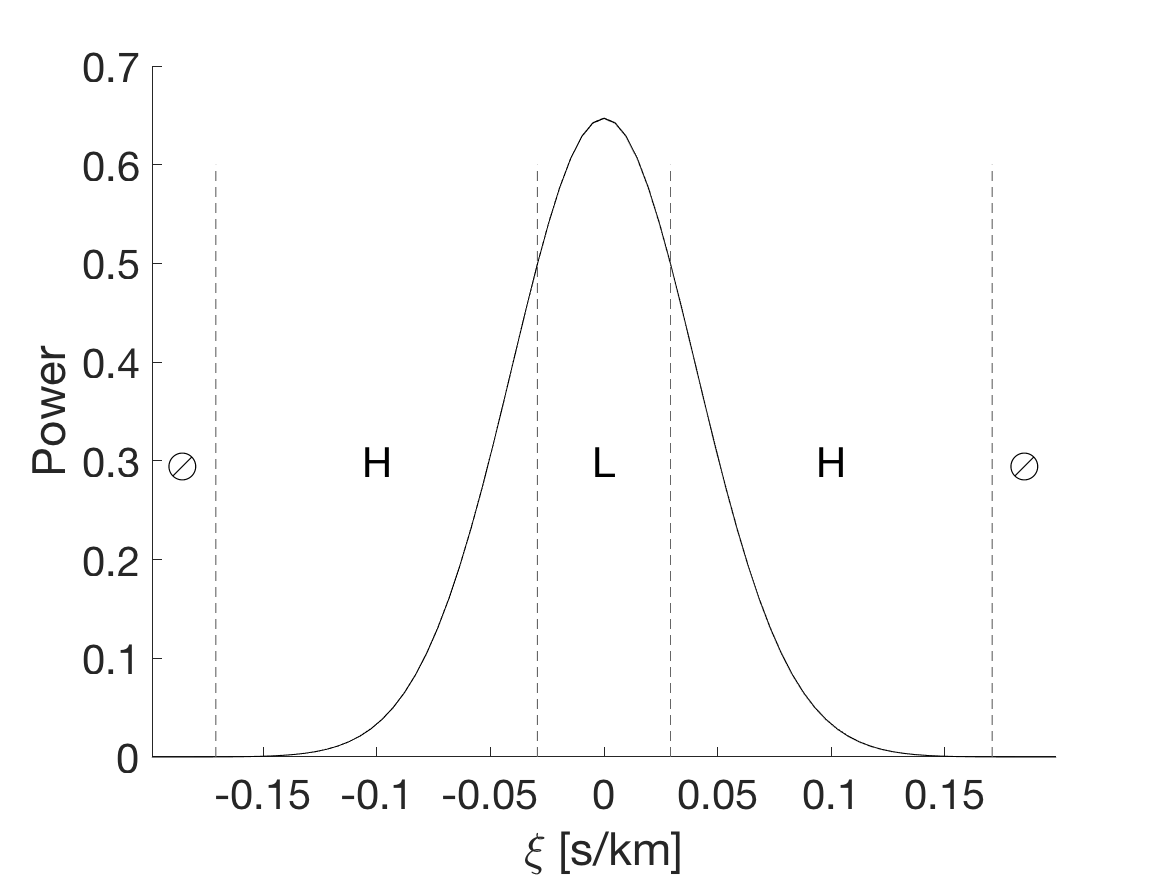
\includegraphics[width=\textwidth]{./Figures/Methods/LPD2-FT_power.png}
        \caption{Power spectrum (stacked)}
    \end{subfigure}
	~
    \begin{subfigure}[b]{0.49\textwidth}
        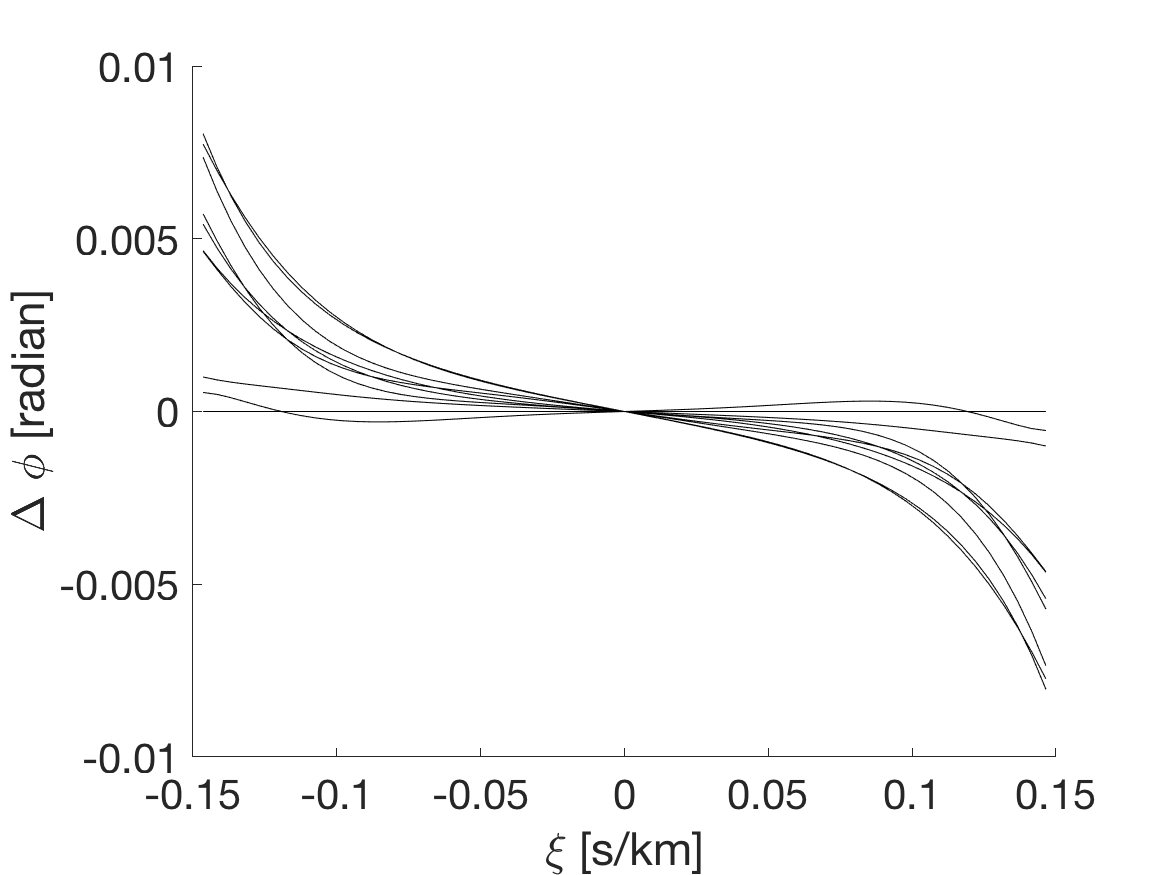
\includegraphics[width=\textwidth]{./Figures/Methods/LPD4-Relative_phase_angle.png}
        \caption{Differential phase spectrum}
        \label{fig:dps_LPD}
    \end{subfigure}	
    
    \caption[Fourier transform of deformed line profiles]
    {Fourier transform of deformed line profiles. Only 10 out of 100 differential phase spectra are presented.}
\label{fig:FT_process_LPD}
\end{figure}    
%-------------

In this case, the input radial velocities would be the apparent radial velocities of deformed line profiles (also known as jitter). Both velocities $RV_\text{FT}$ and $RV_\text{Gaussian}$ are plotted against rotation phase (Fig.~\ref{fig:rv_recovery_deformed}). If we take $\sigma_\text{FT} = \sigma_\text{Gaussian} = 0.08$ m/s to be the intrinsic photon noise level corresponding to S/N = 10,000 as obtained in \S~\ref{sec:Initial_tests}, the difference between $RV_\text{FT}$ and $RV_\text{Gaussian}$ would have an uncertainty of $\sqrt{\sigma_\text{FT}^2+\sigma_\text{Gaussian}^2}\approx0.11$ m/s. What we measure here is $\mid RV_\text{difference}\mid = \mid RV_\text{FT} - RV_\text{Gaussian}\mid < 0.03$ m/s. Therefore, we can agree that $RV_\text{FT}$ and $RV_\text{Gaussian}$ are indistinguishably consistent in the measurement of the apparent radial velocities of a deformed line profile. 

%-------------
\begin{figure}[tbp]
\centering
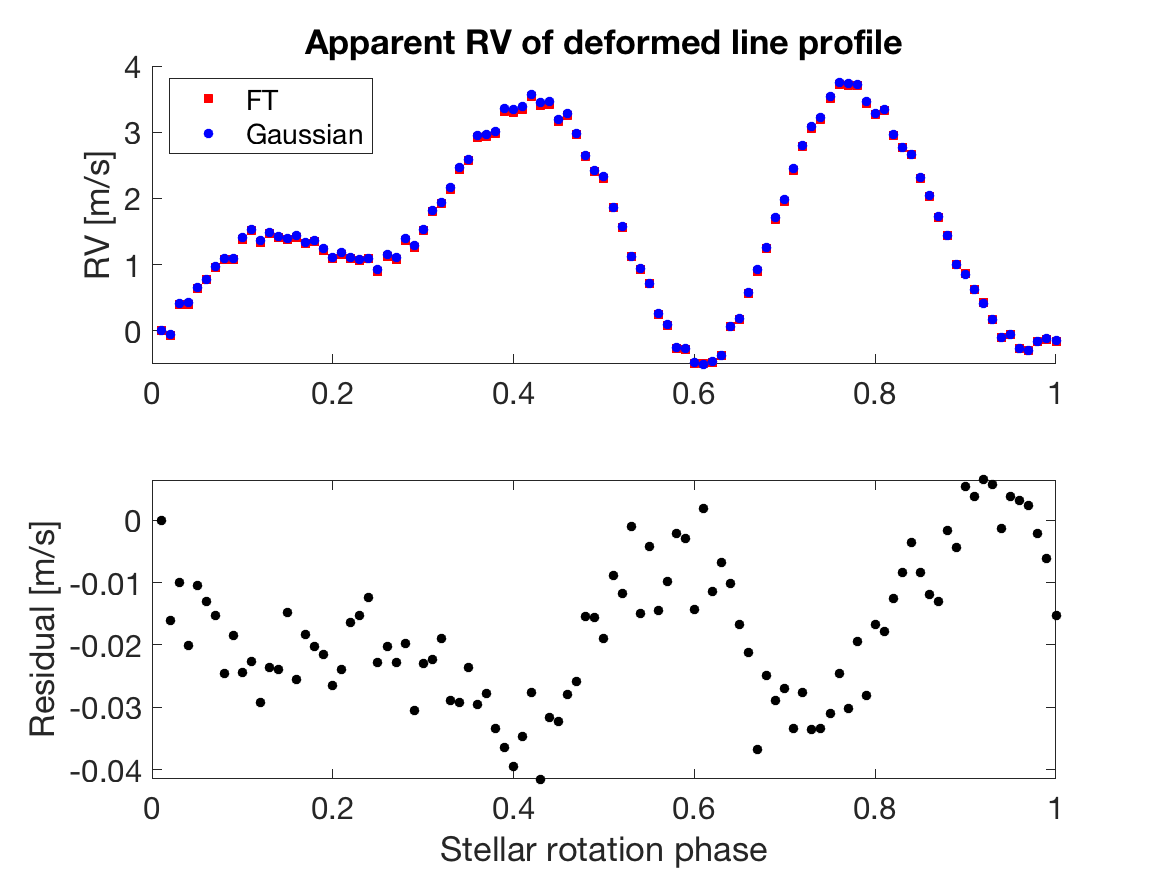
\includegraphics[width = 0.7 \linewidth]
{./Figures/Methods/5-JITTER_ONLY_3.png}
\caption[Apparent RV of deformed line profiles]
{Apparent RV of deformed line profiles calculated with Fourier phase spectrum analysis and Gaussian fit. Both results are also highly consistent with each other. $RV_\text{difference} = RV_\text{FT} - RV_\text{Gaussian}$.}
\label{fig:rv_recovery_deformed}
\end{figure} 
%-------------
\FloatBarrier

%----------------------------------------------------------------------------------------	
\subsubsection{$RV_\text{FT,H}$ and $RV_\text{FT,L}$}
\label{subsec:FT,HL}

Although an intrinsic line deformation (in the absence of any velocity shift in the host star) usually mimics a radial velocity shift, we note the shape differences in the differential phase spectrum between an actual line shift (Fig.~\ref{fig:dps}) and a line deformation (Fig.~\ref{fig:dps_LPD}) -- the latte presents slightly flatter features in lower frequencies and becomes more skewed towards higher frequencies. Such differences provide key messages to differentiate the two circumstances.

According to \S\ref{sec:LD_Theory} where we introduced $\overline{x_0(\xi)}$ -- an averaged shift of a particular frequency range -- we compute the equivalent radial velocity shift for each of the lower and higher frequency ranges (Fig.~\ref{fig:low-high-pass_lpd}). We present our results by plotting the obtained $RV_\text{FT,H/L}$ against the jitter (line centroid fitted by a Gaussian profile) in Fig.~\ref{fig:FT_vs_Gaussian}. The $RV_\text{FT,H}$ and $RV_\text{FT,L}$ are clearly clustered into two groups, both linearly correlated with the jitter, and yet neither has a 1:1 correlation. $RV_\text{FT,H}$ demonstrates a higher response to jitter. Fitting with a linear regression model, it comes with a slope $k_\text{H} = 1.978\pm0.100$, meaning an apparent radial velocity shift of 1 m/s due to line deformation is detected as $1.978\pm0.100$ m/s shift on average using \textit{this} high-pass filter; whereas the slope for applying a low-pass filter is $k_\text{L} = 0.847\pm0.015$, meaning $RV_\text{FT,L}$ is less sensitive to the line profile deformation. It's also worth noting that the combined effect of these two filters would have resulted in $RV_\text{FT}$, a consistent measurement of the radial velocity as with the fitting a line centroid as previously showed.

%-------------
\begin{figure}[tbp]	
    \begin{subfigure}[b]{0.49\textwidth}
        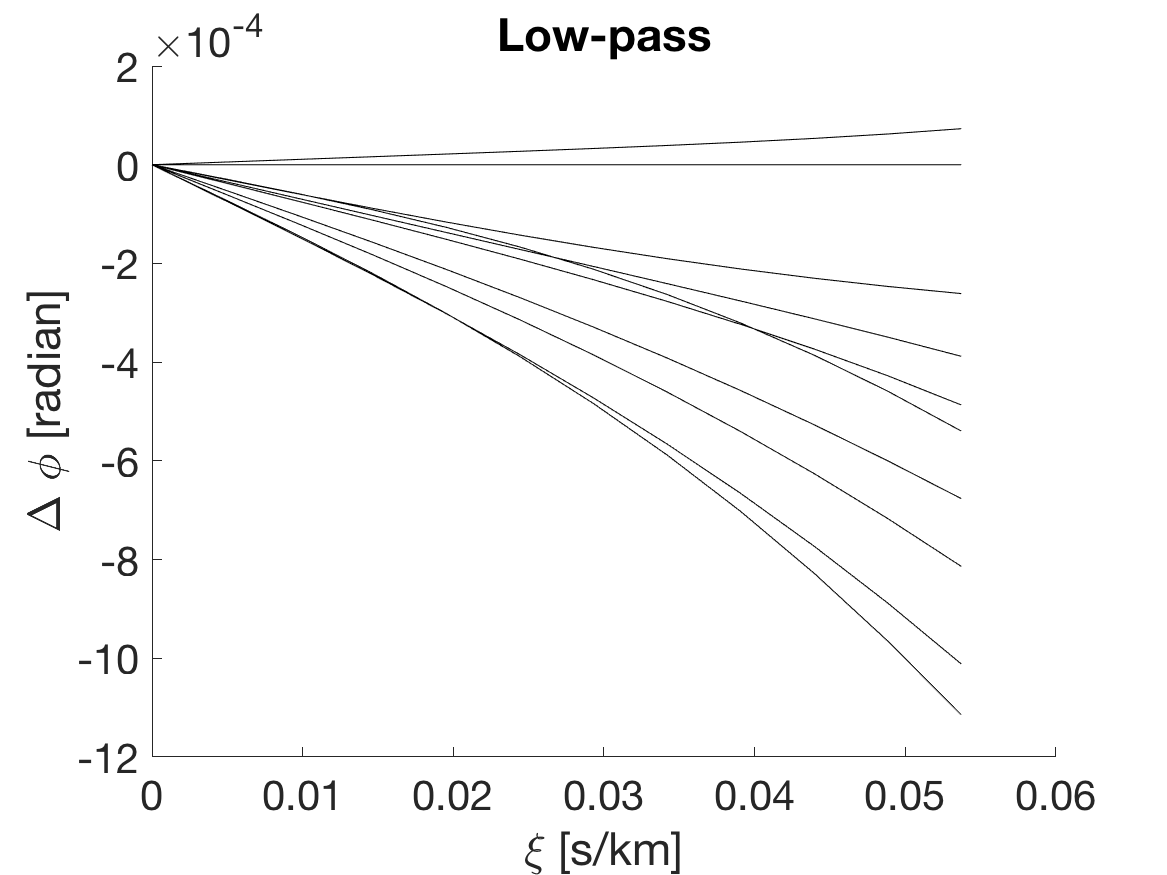
\includegraphics[width=\textwidth]{./Figures/Methods/LPD4-Relative_phase_angle_L.png}
%        \caption{Power spectrum (stacked)}
    \end{subfigure}
	~
    \begin{subfigure}[b]{0.49\textwidth}
        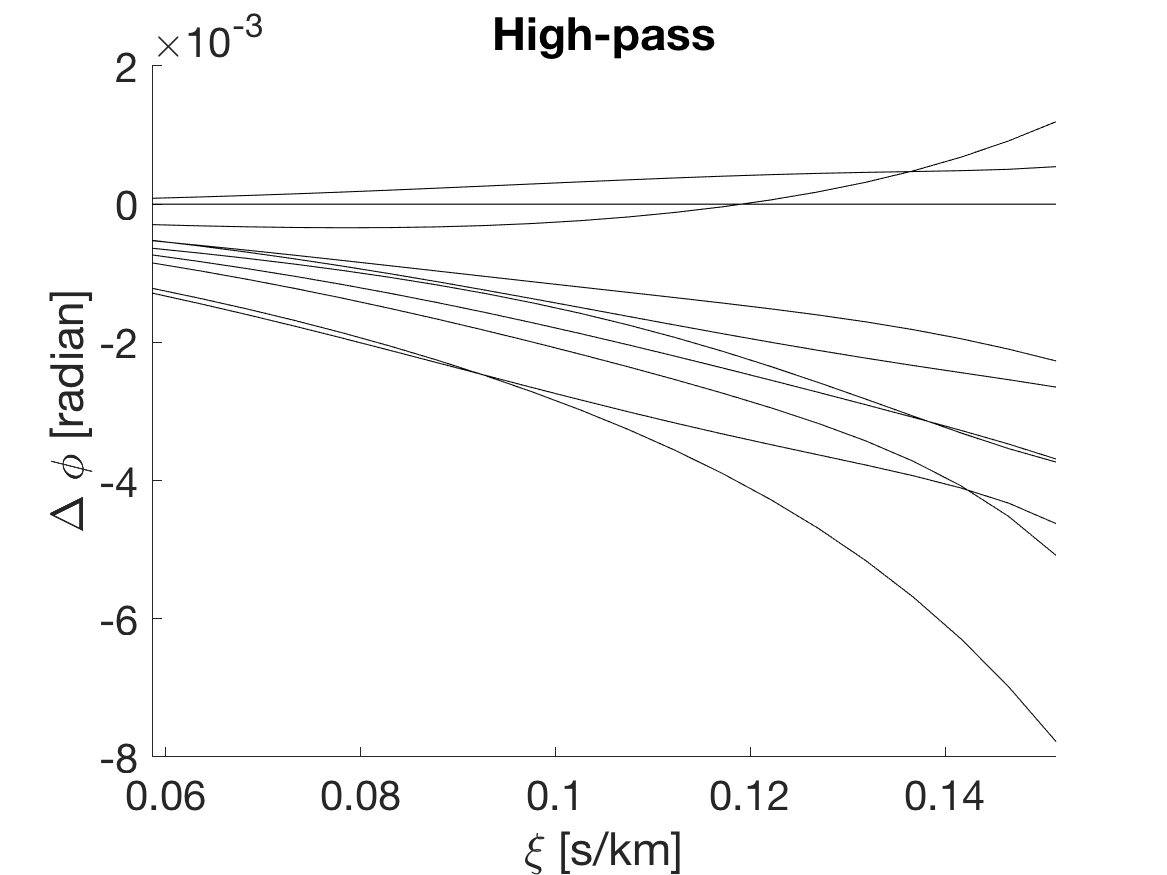
\includegraphics[width=\textwidth]{./Figures/Methods/LPD4-Relative_phase_angle_H.png}
%        \caption{Differential phase spectrum}
    \end{subfigure}	
    
    \caption[Low-pass and high-pass filters]
    {Differential phase spectrum as shown in Fig.~\ref{fig:dps_LPD} sub-divided into lower frequency range and higher frequency range. Only the non-negative ranges are plotted.}
\label{fig:low-high-pass_lpd}
\end{figure}    
%-------------

%-------------
\begin{figure}[tbp]
\centering
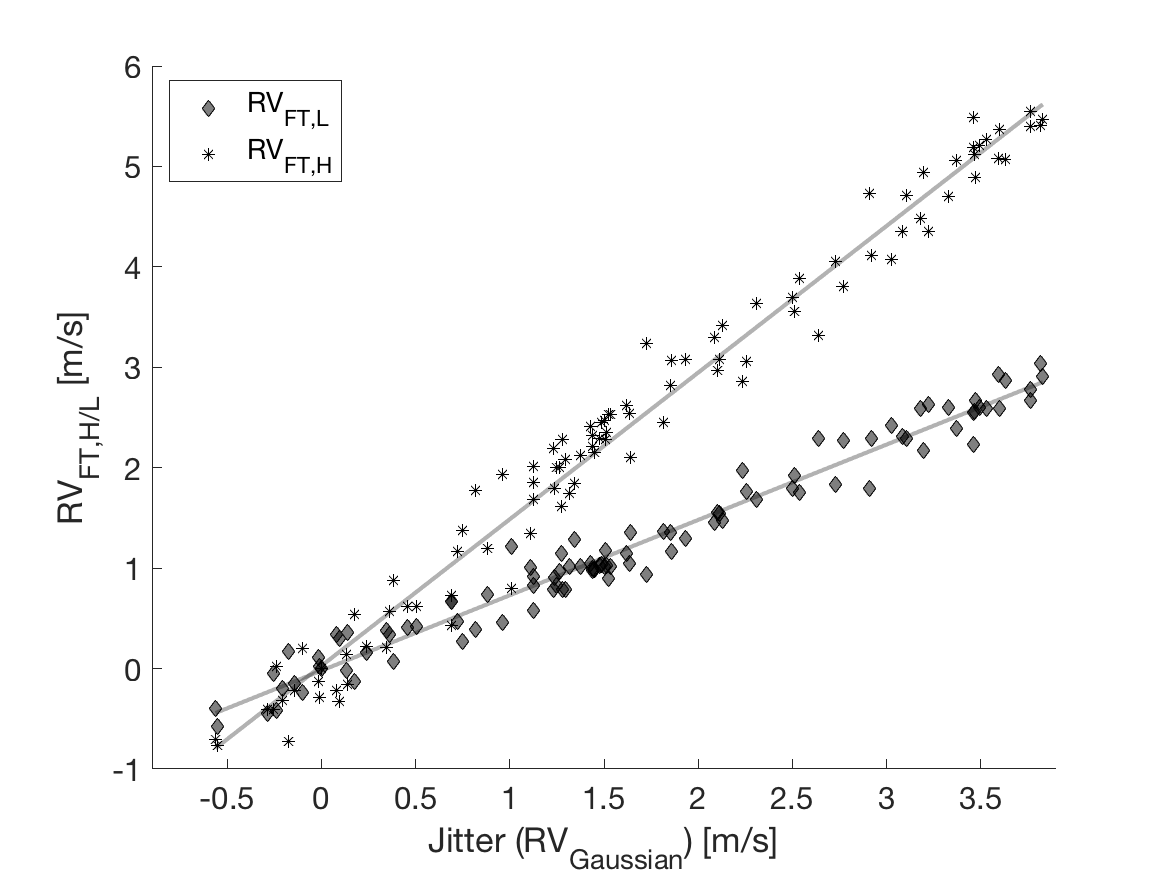
\includegraphics[width = 0.7 \linewidth]
{./Figures/Methods/5-JITTER_ONLY_1.png}
\caption[Fourier transform in response to line deformation]
{Applying the low-pass and high-pass filters, the Fourier transform $RV_\text{FT,L}$ and $RV_\text{FT,H}$ are linearly correlated with the jitter ($RV_\text{Gaussian}$).}
\label{fig:FT_vs_Gaussian}
\end{figure} 
%-------------

We could further investigate how well this linearity behaves for each filter by scaling the measured $RV_\text{FT,L}$ and $RV_\text{FT,H}$ by their corresponding factors $1/k_\text{L}$ and $1/k_\text{H}$ respectively, and compare them with the jitter ($RV_\text{Gaussian}$), as presented in Fig.~\ref{fig:scaling_RV_FT}. The root-mean-squares of the residuals are $\sigma_\text{FT,L} \approx 0.11$ m/s and $\sigma_\text{FT,H} \approx 0.31$ m/s respectively. The reason for $\sigma_\text{FT,H}>\sigma_\text{FT,L}$ is the same as mentioned in \S\ref{sec:Further_tests}, being higher frequency modes are more sensitive to noise, but the fact that both $\sigma_\text{FT,H/L}$ increase (opposed to $\sigma_\text{FT,H/L}$ = 0.08~m/s in the case of a pure line shift) is because we think the linearity between $RV_\text{FT,H/L}$ and the input jitter is only empirically valid but not strictly followed. The deviation from linearity would affect how well we could recover the jitter by scaling $RV_\text{FT,H/L}$ and may also introduce systematics in the recovery of jitter. 

%-------------
\begin{figure}[tbp]
\centering
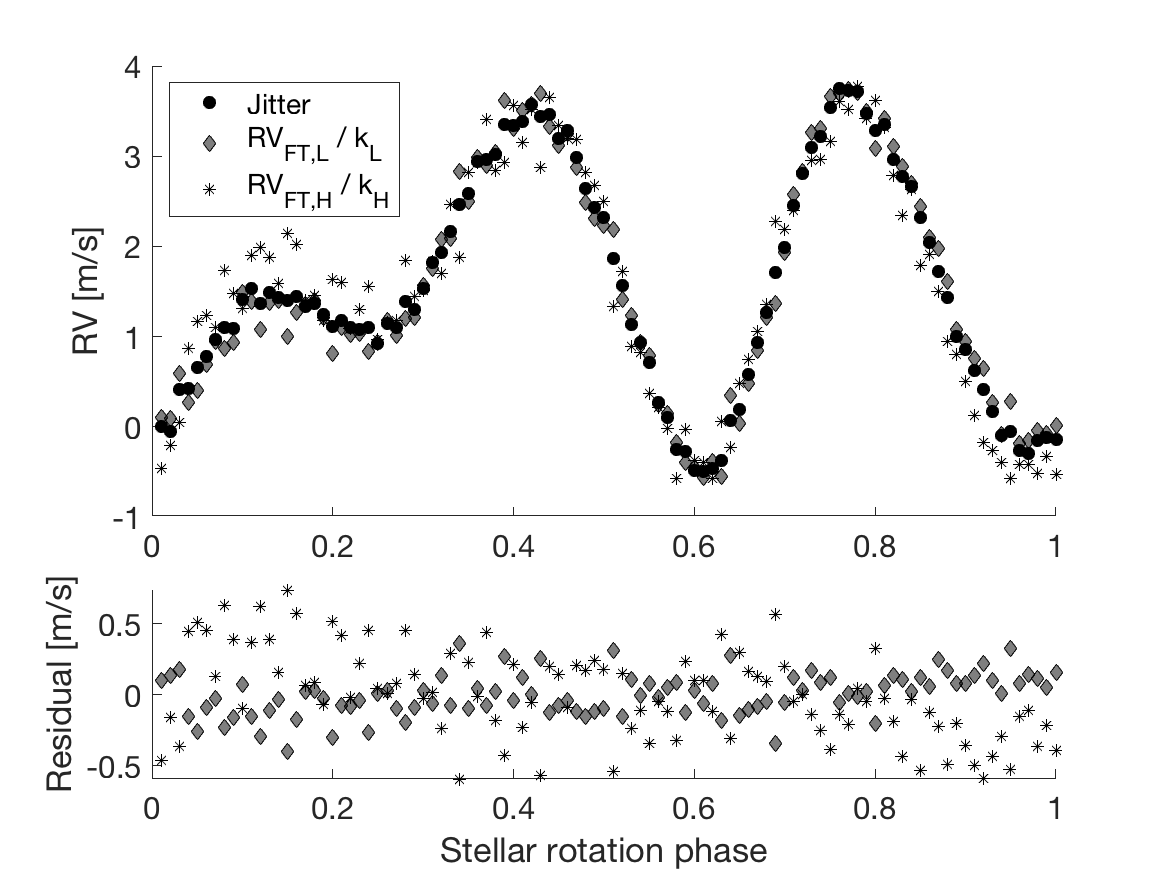
\includegraphics[width = 0.7 \linewidth]
{./Figures/Methods/5-JITTER_ONLY_4.png}
\caption[Scaling the low-pass and high-pass Fourier transformed radial velocities]
{Scaling the low-pass and high-pass Fourier transformed radial velocities to match the input jitter.}
\label{fig:scaling_RV_FT}
\end{figure} 
%-------------

%----------------------------------------------------------------------------------------	
\subsection{Jitter model}
\label{subsec:Jitter_model}

We have shown in \S~\ref{ch:FT_line_shift} that the following measurable quantities demonstrate basically the same response to pure line shifts: $RV_\text{FT}$, $RV_\text{FT,H/L}$ and $RV_\text{Gaussian}$. We have also shown in this section (\S~\ref{sec:FT_ld}) so far, that both $RV_\text{FT,H}$ and $RV_\text{FT,L}$ are linearly correlated with the jitter, to which $RV_\text{FT,H}$ is more sensitive ($k_\text{H}>1$) and $RV_\text{FT,L}$ is less sensitive ($k_\text{L}<1$). 

We can therefore write the following measurable quantities -- $RV_\text{Gaussian}$ (or $RV_\text{FT}$), $RV_\text{FT,L}$ and $RV_\text{FT,H}$ -- in the from of three additive terms: (1) a bulk shift in the star (which we hereafter assume to be due to a planet or planets) as the superposition of Keplerian orbit(s), (2) variability in the stellar line profile (hereafter lumped under the general name ``jitter''), and (3) a constant radial velocity offset term that we choose it to be absorbed into the previous two terms for elegance.
\begin{align}
	RV_\text{Gaussian} 	&= RV_\text{planet} + RV_\text{jitter}				 \label{eq:RV_Gau} \\
	RV_\text{FT,L} 		&= RV_\text{planet} + k_L \cdot RV_\text{jitter} 		 \label{eq:RV_FTL} \\
	RV_\text{FT,H} 		&= RV_\text{planet} + k_H \cdot RV_\text{jitter}.		 \label{eq:RV_FTH}
\end{align}
Subtracting one from the other to remove $RV_\text{planet}$ and reduce to two independent equations
\begin{align}
	RV_\text{Gaussian} - RV_\text{FT,L} 	&= (1-k_L) \cdot RV_\text{jitter}\\
	RV_\text{FT,H} - RV_\text{Gaussian}	&= (k_H-1) \cdot RV_\text{jitter}
\end{align}
Rearranging yields two expressions of the jitter model
\begin{align}
	RV_\text{jitter} &= \frac{RV_\text{Gaussian} - RV_\text{FT,L}}{1-k_L} 	\label{eq:jitter_model1} \\
	RV_\text{jitter} &= \frac{RV_\text{FT,H} - RV_\text{Gaussian}}{k_H-1}		\label{eq:jitter_model2} 
\end{align}
where $RV_\text{Gaussian}, RV_\text{FT,L}$ and $RV_\text{FT,H}$ are direct measurements, whereas $k_L$ and $k_H$ are unknowns -- we could determine $k_L$ and $k_H$ in the previous demonstrated simulations only because we knew there was no other radial velocities than jitter in the system. Dividing the two equations above further cancels $RV_\text{jitter}$, leaving 
\begin{equation}
	\frac{RV_\text{Gaussian}-RV_\text{FT,L}}{RV_\text{FT,H} - RV_\text{Gaussian}} = \frac{1-k_L}{k_H-1},
\label{eq:GHL} 
\end{equation}
which means $(1-k_L)/(1-k_H)$ can now be robustly obtained by fitting a linear regression model on $(RV_\text{Gaussian}-RV_\text{FT,L})$ against $(RV_\text{Gaussian} - RV_\text{FT,H})$. With this, we rewrite the jitter model in a unified form -- the weighted sum of the two jitter expressions from Eq.~\ref{eq:jitter_model1} and Eq.~\ref{eq:jitter_model2}: 
\begin{align*}
	RV_\text{jitter} &= w_1 \frac{RV_\text{Gaussian} - RV_\text{FT,L}}{1-k_L} + w_2 \frac{RV_\text{FT,H}-RV_\text{Gaussian}}{k_H-1} \\
	&= \frac{1}{{k_H-1}} \bigg[w_1 \frac{RV_\text{Gaussian} - RV_\text{FT,L}}{\frac{1-k_L}{k_H-1}} + w_2 (RV_\text{FT,H}-RV_\text{Gaussian})\bigg] \\
	&= \alpha \bigg[w_1 \frac{RV_\text{Gaussian} - RV_\text{FT,L}}{\frac{1-k_L}{k_H-1}} + w_2 (RV_\text{FT,H}-RV_\text{Gaussian})\bigg] \numberthis \label{eq:jitter_model_final}
\end{align*}
in which the weights satisfy $w_1+w_2=1$ and $1/(k_H-1)$ is replaced by the scaling factor $\alpha$ in the last step. 

%Additionally, we can roughly estimate the uncertainty of $RV_\text{jitter}$ in Eq.~\ref{eq:jitter_model1} and Eq.~\ref{eq:jitter_model2} by treating $RV_\text{Gaussian}$, $RV_\text{FT,L}$ and $RV_\text{FT,H}$ are independent variables, and $k_{L/H}$ is a constant: 
%\begin{align}
%	\Delta RV_\text{jitter,L} &\approx \frac{\sqrt{\sigma_\text{Gaussian}^2 + \sigma_\text{FT,L}^2}}{1-k_L} \\
%	\Delta RV_\text{jitter,H} &\approx \frac{\sqrt{\sigma_\text{Gaussian}^2 + \sigma_\text{FT,H}^2}}{k_H-1}.
%\end{align}
%Substituting the following values: $\sigma_\text{Gaussian} = 0.08$ m/s (\S\ref{sec:Initial_tests}), $\sigma_\text{FT,L} = 0.11$ m/s and $\sigma_\text{FT,H} = 0.43$ m/s (\S\ref{sec:Further_tests}), $k_L = 0.847$ and $k_H = 1.978$ (\S\ref{subsec:FT,HL}), we obtain $\Delta RV_\text{jitter,L} = 0.89$ m/s and $\Delta RV_\text{jitter,H} = 0.45$ m/s.

As a final remark, we strongly suggest check the correlation between $(RV_\text{Gaussian}-RV_\text{FT,L})$ and $(RV_\text{FT,H} - RV_\text{Gaussian})$ from Eq.~\ref{eq:GHL} before going ahead with the jitter model (Eq.~\ref{eq:jitter_model1} and Eq.~\ref{eq:jitter_model2}), because our jitter model is solely based on the empirically assumed linear response of $RV_\text{FT,H/L}$ to $RV_\text{jitter}$, either of which fails can be identified by plotting $(RV_\text{Gaussian}-RV_\text{FT,L})$ against $(RV_\text{FT,H} - RV_\text{Gaussian})$.

%----------------------------------------------------------------------------------------	
\subsection{Testing the recovery of jitter}
\label{sec:check}

We again performed tests to demonstrate we could correctly recover artificially generated jitter using our new technique (Eq.~\ref{eq:jitter_model_final}). We generated 200 deformed line profiles (in the form of cross-correlation functions) using SOAP~2.0. All the configurations are the same as used in \S\ref{sec:Simulations}, except that the data are produced from two rotation periods instead of one. The jitter amplitude is roughly 2 m/s. In addition, each line profile is further shifted by an amount $RV_\text{planet}$ with an amplitude of the Keplerian orbit $A_\text{planet} = 2~\text{m/s}$ (although in principle the $RV_\text{planet}$ configuration shouldn't affect the jitter model because the term was cancelled out when we derived the jitter expression). The planetary orbital frequency to stellar rotation frequency ratio is set to be 0.7 (i.e. $\nu_\text{orb}/\nu_\text{rot} = P_\text{rot}/P_\text{orb} = 0.7$). 

We then obtain three sets of radial velocities for each simulated profile: $RV_\text{Gaussian}$, $RV_\text{FT,H}$ and $RV_\text{FT,L}$ (Fig.~\ref{fig:PLANET_AND_JITTER} upper panel). We test three different combinations of $w_1$ and $w_2$ and apply a scaling factor $\alpha$ (fitted by linear regression to the known input jitter) to see how well it matches the input jitter: (1) $w_1=1, w_2=0$; (2) $w_1=0.5, w_2=0.5$; (3) $w_1=0, w_2=1$. It shows in the middle panel, that all these three sets of jitter model successfully recover adequate information of the input jitter, while presenting minor difference among each other. 

%-------------
\begin{figure}[tbp]
\centering
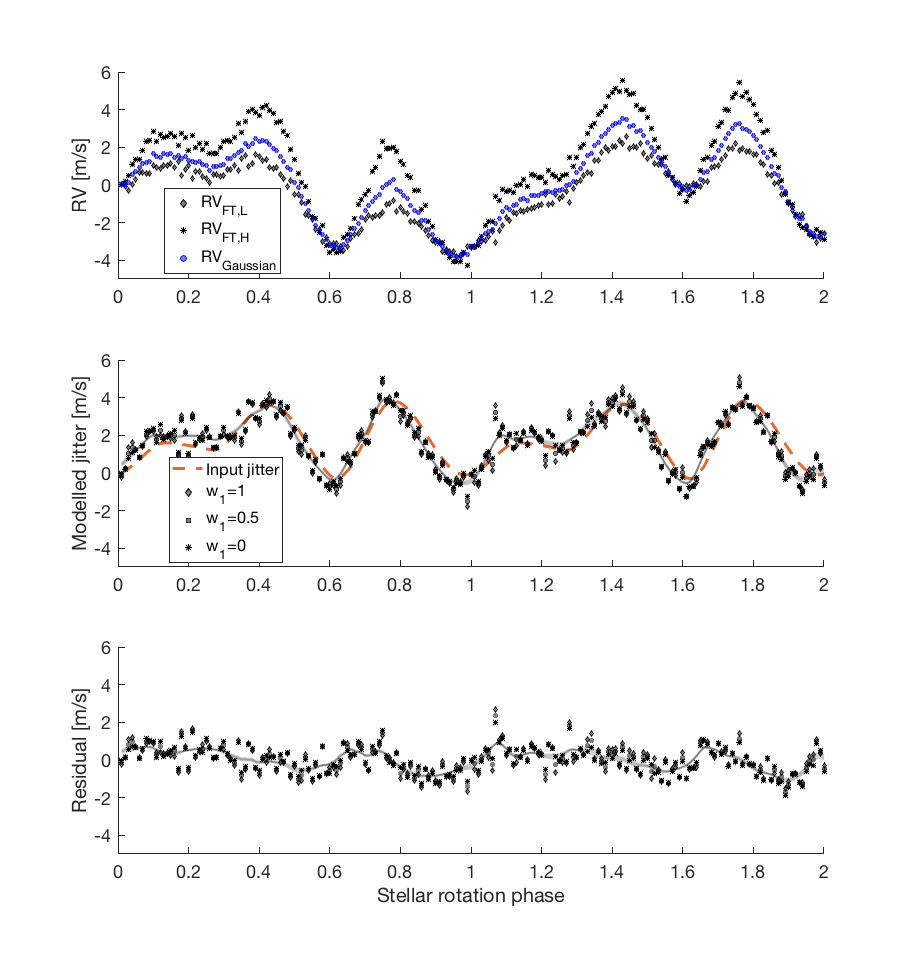
\includegraphics[width = 0.99 \linewidth]
{./Figures/Methods/5-PLANET_AND_JITTER2.png}
\caption[Jitter model]
{Jitter recovery based on Eq.~\ref{eq:jitter_model_final} for the simulated data (S/N = 10,000). Top: time series of directly measured $RV_\text{Gaussian}$ and $RV_\text{FT,H/L}$. Middle: three forms of jitter expression scaled by their respective factor $\alpha$, smoothed by the weighted moving average (mostly overlapping grey solid line) with $\tau = 0.01 P_{rot}$. In comparison is the input jitter (orange dashed line). Bottom: difference between the jitter model and the input jitter, smoothed by the weighted moving average (mostly overlapping grey solid line).}
\label{fig:PLANET_AND_JITTER}
\end{figure} 
%-------------

\paragraph{Weighted moving average} At this stage, we would implement a weighted moving average modulated by a Gaussian kernel to mitigate noise brought by $RV_\text{FT,H/L}$ (excessive noise due to the sacrifice of frequency information) and the subsequent arithmetic. For $N$ data points (e.g. radial velocities) $v_i$ with an uncertainty $\sigma_i$ observed at $t_i$ ($i=1,2,...N$), we define the contribution (i.e. weight) of a data point $(t_i, v_i\pm \sigma_i)$ towards the chosen position $t$ as the multiplication of two factors: (1) the weight of the data point itself, inversely proportional to the uncertainty squared: $W_i= \frac{1}{\sigma_i^2}$ and (2) a stationary kernel that describes the correlation between data, depending on the distance $\mid t-t_i \mid$ and a time-scale of correlation $\tau$: $K_i(t) = e^{-\frac{(t-t_i)^2}{2\tau^2}}$. With this, the evaluation of a data point $v(t)$ can be drawn by the weighted average of all observed data $(t_i, v_i\pm \sigma_i)$, with the weight 
\begin{equation}
	\textbf{W}_i(t) = W_i \cdot K_i(t) = \frac{1}{\sigma_i^2} e^{-\frac{(t-t_i)^2}{2\tau^2}}
\end{equation}
respectively and then normalised by the sum of weights, so that 
\begin{equation}
	v(t) 	=  \frac{\sum\limits_{i=1}^{N} \bigg[x_i*\textbf{W}_i(t)\bigg]}{\sum\limits_{i=1}^{N} \textbf{W}_i(t)}
\end{equation}

To quantitatively examine their performance, we compare the scatter of the difference between the input jitter and the jitter models -- $\sigma_\text{residual}$ -- with the scatter of the input jitter -- $\sigma_\text{jitter} = 1.22$~m/s. The former can be treated as the scatter after the planets are correctly fitted and jitter is removed, whereas the latter the scatter after fitting the correct planet(s) without jitter correction. Table~\ref{table:jitter_model_scatter} lays out the scatter $\sigma_\text{residual}$ for the raw jitter models and the smoothed jitter models implemented with the weighted moving average. In addition to the nearly noise-free (S/N=10,000) simulations, the corresponding simulations appropriate for real-world observations are presented in parallel. For example, S/N of the cross-correlation line profile close to 10,000 are found in $\alpha$ Cen B observations from HARPS; S/N ranging from 2,000 to 4,000 are found in a dwarf star HD~189733, whose apparent magnitude is $V=7.6$; S/N$\sim$1,000 is found for red dwarfs Gl~176 and Wolf~1061, of which $V\sim10$. 

%-------------
\begin{table}[htbp]
\centering
\begin{tabular}{|c|c|c|c|c|}
\hline
\multirow{2}{*}{} 	& \multicolumn{2}{c|}{$\sigma_\text{residual}$ (raw) [m/s]}  & \multicolumn{2}{c|}{$\sigma_\text{residual}$ (smoothed) [m/s]}  \\ \cline{2-5} 
                  	& \multicolumn{1}{l|}{S/N=10,000} & \multicolumn{1}{l|}{S/N=2,000} & \multicolumn{1}{l|}{S/N=10,000} & \multicolumn{1}{l|}{S/N=2,000} \\ \hline
$w_1=1, w_2=0$  	 	& 0.69 		& 2.49 			& 0.54 			& 0.65                              \\ \hline
$w_1=0.5, w_2=0.5$  & 0.78 		& 2.59			& 0.62			& 0.75                              \\ \hline
$w_1=0, w_2=1$      & 0.72		& 2.42			& 0.51 			& 0.68                              \\ \hline
\end{tabular}
\caption{Scatter of jitter residual (input $\sigma_\text{jitter} = 1.22$~m/s)}
\label{table:jitter_model_scatter}
\end{table}
%-------------

We note from the table, that the scatter of the input jitter is effectively reduced from 1.22~m/s to $\sigma_\text{residual} = 0.70$~m/s for S/N=10,000 but conversely doubled for S/N=2,000. Implementing the weighted moving average with a proper correlation time-scale $\tau$ (e.g. depend on the detail of information to be extracted from the data and the extent of noise to be flattened) can reduce the input jitter scatter $\sigma_\text{jitter}$ by half in both cases. In this exercise, we choose the correlation time-scale for S/N=10,000 to be $\tau_{10000} = 0.01 P_{rot}$, the distance between two cadence of simulated observations, and $\tau_{2000} = 5~\tau_{10000}$ for S/N=2,000 in order to further mitigate noise. We have also tested other smoothing approaches, such as the use of the Python package PyMC3 that implements Gaussian process in smoothing the data, which also returns similarly results. 

Reaching sub-m/s in the residuals of fitting the jitter indicate the our potential to enhance the detection of planets in sub-m precisions (as long as the instrument allows, stellar variability won't be a barrier) and reveal candidates with radial velocities of sub-m/s amplitudes. However, this would require good sampling and we should not ignore there can be systematic differences between the input jitter and our jitter models.

%----------------------------------------------------------------------------------------
\subsection{Planetary radial velocity recovery}

In this subsection we discuss the possibilities to recover the radial velocity of the planet in a more direct way, though may not be as practical.

Having obtained the jitter model (Eq.~\ref{eq:jitter_model_final}) and knowing $RV_\text{planet}$ follows a Keplerian orbital motion, we can turn our planetary radial velocity recovery into a model fitting problem, in which the parameters of the jitter model (such as the scaling factor) and that of the Keplerian orbit (such as amplitude, orbital period and phase) are to be determined. 

Alternatively, we can bypass the jitter model. Revisiting the Equations \ref{eq:RV_Gau}-\ref{eq:RV_FTH}, we rewrite them by observation number $i (i=1,2,\ldots,N)$ and switch the notations to obtain the following $3N$ independent linear equations:
\begin{align}
	X_i 		&= P_i + J_i				\label{eq:XX} \\
	Y_i 		&= P_i + k_y \cdot J_i	\label{eq:YY} \\
	Z_i 		&= P_i + k_z \cdot J_i 	\label{eq:ZZ}
\end{align}
where $X_i, Y_i$ and $Z_i$ replace the three measurable radial velocities $RV_\text{Gaussian}$, $RV_\text{FT,L}$ and $RV_\text{FT,H}$; $P_i$ and $J_i$ are the planetary radial velocities and the jitter; $k_y$ and $k_z$ are the scaling factors $k_L$ and $k_H$. Substituting $J_i = X_i - P_i$ from Eq.~\ref{eq:XX}, we can simplify the system to the following $2N$ independent linear equations:
\begin{align}
	Y_i 		&= k_y \cdot X_i + (1-k_y)P_i	\label{eq:YYY} \\
	Z_i 		&= k_z \cdot X_i + (1-k_z)P_i	\label{eq:ZZZ}.
\end{align}
The number of unknowns is $(N+4)$, including $N$ from $P_i$, 2 from $k_y$ and $k_z$, and another 2 from the previously absorbed constant offsets. Normally we have $N \gg 1$, so that the number of independent equations ($2N$) is larger than the number of degrees of freedom $(N+4)$ in the system, meaning the system can be uniquely solved by optimization, such as least square minimization of the objective function:
\begin{equation}
	\sum_{i=1}^{N} \Bigg[w_{y,i}\Big(k_y \cdot X_i + (1-k_y)P_i - Y_i \Big)^2 + w_{z,i}\Big(k_z \cdot X_i + (1-k_z)P_i- Z_i \Big)^2 \Bigg]
\label{eq:objective_function}
\end{equation}
where $w_{y,i}$ and $w_{z,i}$ are pre-determined parameters (e.g. determined by the sizes of errorbars of the observed radial velocities) used to weight the linear systems. In addition, this approach becomes identical to constructing a jitter model (Eq.~\ref{eq:jitter_model_final}) in cases that (1) $w_{y,i}=1, w_{z,i}=0 (i=1,2,\ldots,N)$ and $w_1=1, w_2=0$; (2) $w_{y,i}=0, w_{z,i}=1 (i=1,2,\ldots,N)$ and $w_1=0, w_2=1$. 

\subsection{Conclusion}

The Fourier phase spectrum analysis, when using (almost) all the information in the power spectrum and the phase spectrum, returns highly consistent radial velocities as the line centroid acquired by fitting a Gaussian profile. This consistency applies both for measuring a direct line shift and an apparent shift of a deformed line profile. 

We believe the frequency dependent $x_0(\xi)$ is the key asset to identifying line profile deformation and distinguishing it from a bulk shift of a line. As far as we have investigated for a deformed line profile, the apparent radial velocity shift (i.e. jitter) can be seen as a mingle of two radial velocities -- $RV_\text{FT,H}$ and $RV_\text{FT,L}$ -- one in higher frequency modes the other in lower frequency modes. They are both, as obtained from the simulated spectral line profiles, scaled linearly with jitter. 

The different linear responses of $RV_\text{FT,H}$ and $RV_\text{FT,L}$ enable us to construct a jitter model, which has reasonably recovered the simulated radial velocity data with stellar variability, both in our almost noise-free and real-world simulations. 

\pagebreak
%----------------------------------------------------------------------------------------	
%----------------------------------------------------------------------------------------	
\section{End-to-end simulations}
\label{\thesection}
\label{sec:end-to-end}

We run end-to-end simulations of recovering a planet candidate in the presence of jitter through to answer the following three questions:
\begin{enumerate}
	\item In a system where the amplitude of jitter is comparable to that of the planetary radial velocities, can we recover the planet orbital parameters better with our Fourier phase spectrum analysis than without jitter correction? 
	\item In a system where the planetary radial velocities dominate and jitter is negligible, does the Fourier phase spectrum analysis give at least equally good results as the traditional methods? 
	\item In a system where jitter is the only source of radial velocities, can it be classified by the Fourier phase spectrum analysis?
\end{enumerate}

The spectral line profile simulator setup is the same as previously. The jitter amplitude is fixed at roughly 2~m/s, so we will adjust the planetary orbital amplitude to satisfy the three categories of end-to-end simulations. For S/N, we choose two numbers to represent the simulations: (1) S/N = 10,000 for super bright stars, where we will show its ability to make significant improvement using the Fourier phase spectrum analysis on recovering the planetary signals when the star is active; (2) S/N = 2,000 where it starts to push the limit of the Fourier phase spectrum analysis. We will run 500 trails, each trail with 60 randomly selected samples clustered in 12 groups, out of a total of 400 equally spaced samples from four stellar rotation periods. 

The tests are divided into two main groups for comparison:
\begin{enumerate}
	\item Fit $RV_\text{Gaussian}$ by Keplerian orbit alone;
	\item Fit $RV_\text{Gaussian}$ by Keplerian orbit with jitter model correction. The following three variations of model fitting have been tested:
   \begin{enumerate}
     \item Jitter model constructed with $RV_\text{Gaussian}$ and $RV_\text{FT,L}$ only, i.e. $w_1=1$ and $w_2=0$;
     \item Jitter model constructed with $RV_\text{Gaussian}$ and $RV_\text{FT,H}$ only, i.e. $w_1=0$ and $w_2=1$;
     \item Jitter model constructed with $RV_\text{Gaussian}$, $RV_\text{FT,L}$ and $RV_\text{FT,H}$. We test with $w_1=0.5$ and $w_2=0.5$.
   \end{enumerate}
\end{enumerate}
The parameters for the fitting is obtained by Markov chain Monte Carlo (MCMC) sampling. Each radial velocity data is equally weighted as they have the same S/N in our simulation. We find that among the three variations of jitter correction treatments, the one left with the least rms empirically returns the best fitting parameters, so we will choose the one to represent the fitting from Group~2. 

%----------------------------------------------------------------------------------------
\subsection{Stellar jitter as strong as planetary signal}

The injected planet has the same parameter settings as in \S\ref{sec:check}, i.e. circular orbit with amplitude $A = 2$~m/s,
orbital frequency ratio $\nu = \nu_\text{orb}/\nu_\text{rot}= 0.7$ and initial phase $\omega = 1$~rad. We recover the parameters for each trail (such as shown in Fig.~\ref{fig:Corner}) for a total of 500 runs and obtain the histograms of the recovered orbital parameters, and present the amplitude and the orbital frequency ratio (inverse of the orbital period ratio) that we are mostly concerned about in Fig.~\ref{fig:Histogram}. 

%-------------
\begin{figure}[tbp]	
    \begin{subfigure}[b]{0.49\textwidth}
        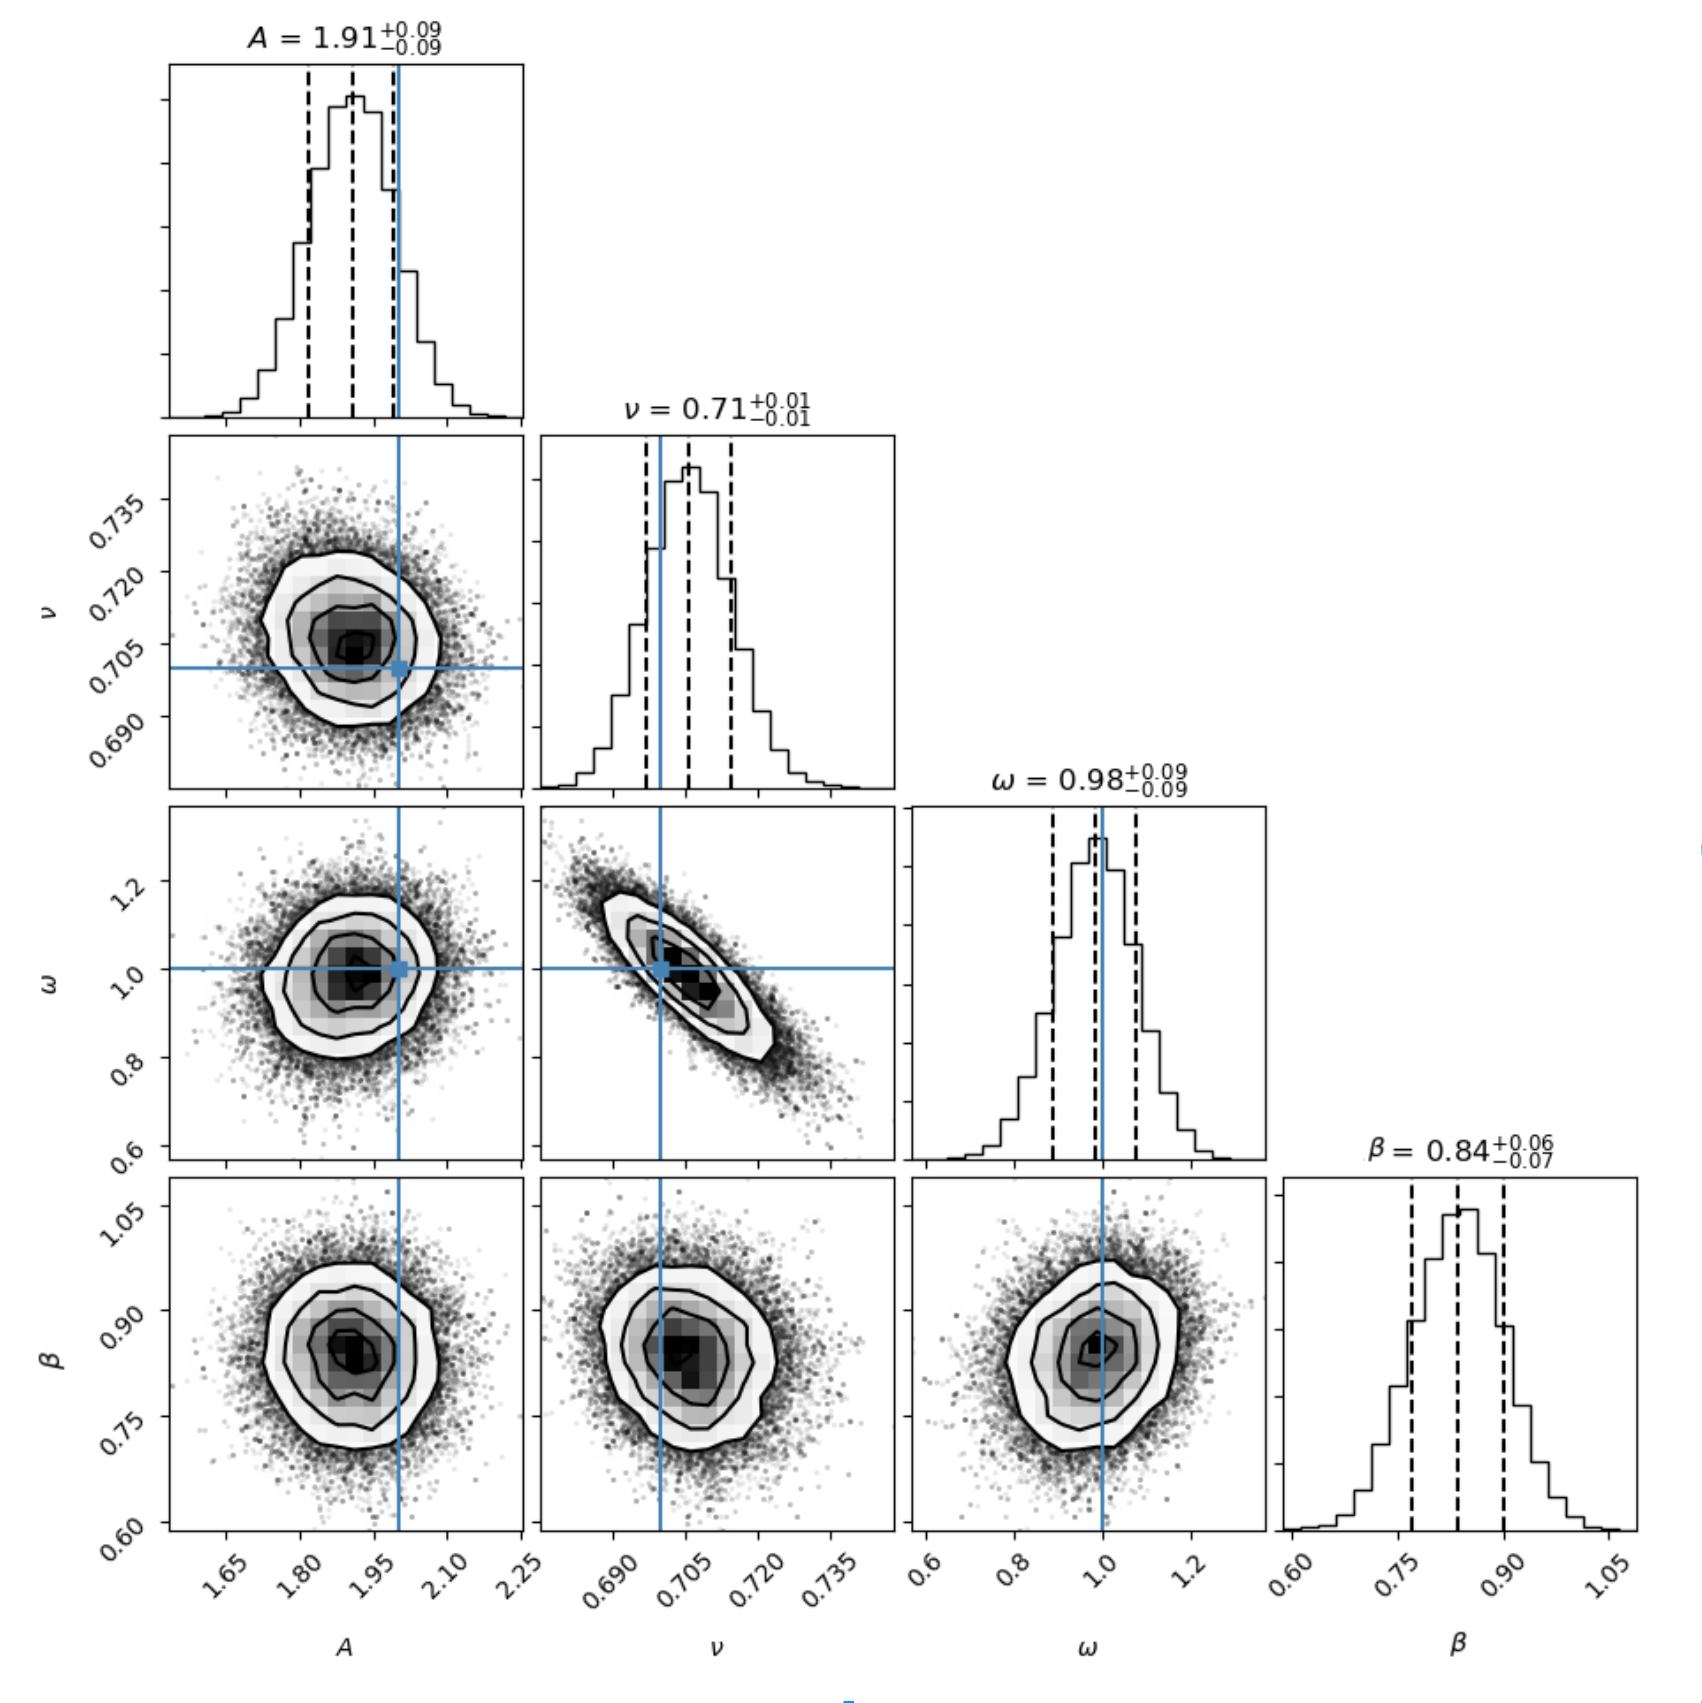
\includegraphics[width=\textwidth]{./Figures/Methods/Fitting_3-MCMC2.png}
        \caption{No jitter correction}
    \end{subfigure}
	~
    \begin{subfigure}[b]{0.49\textwidth}
        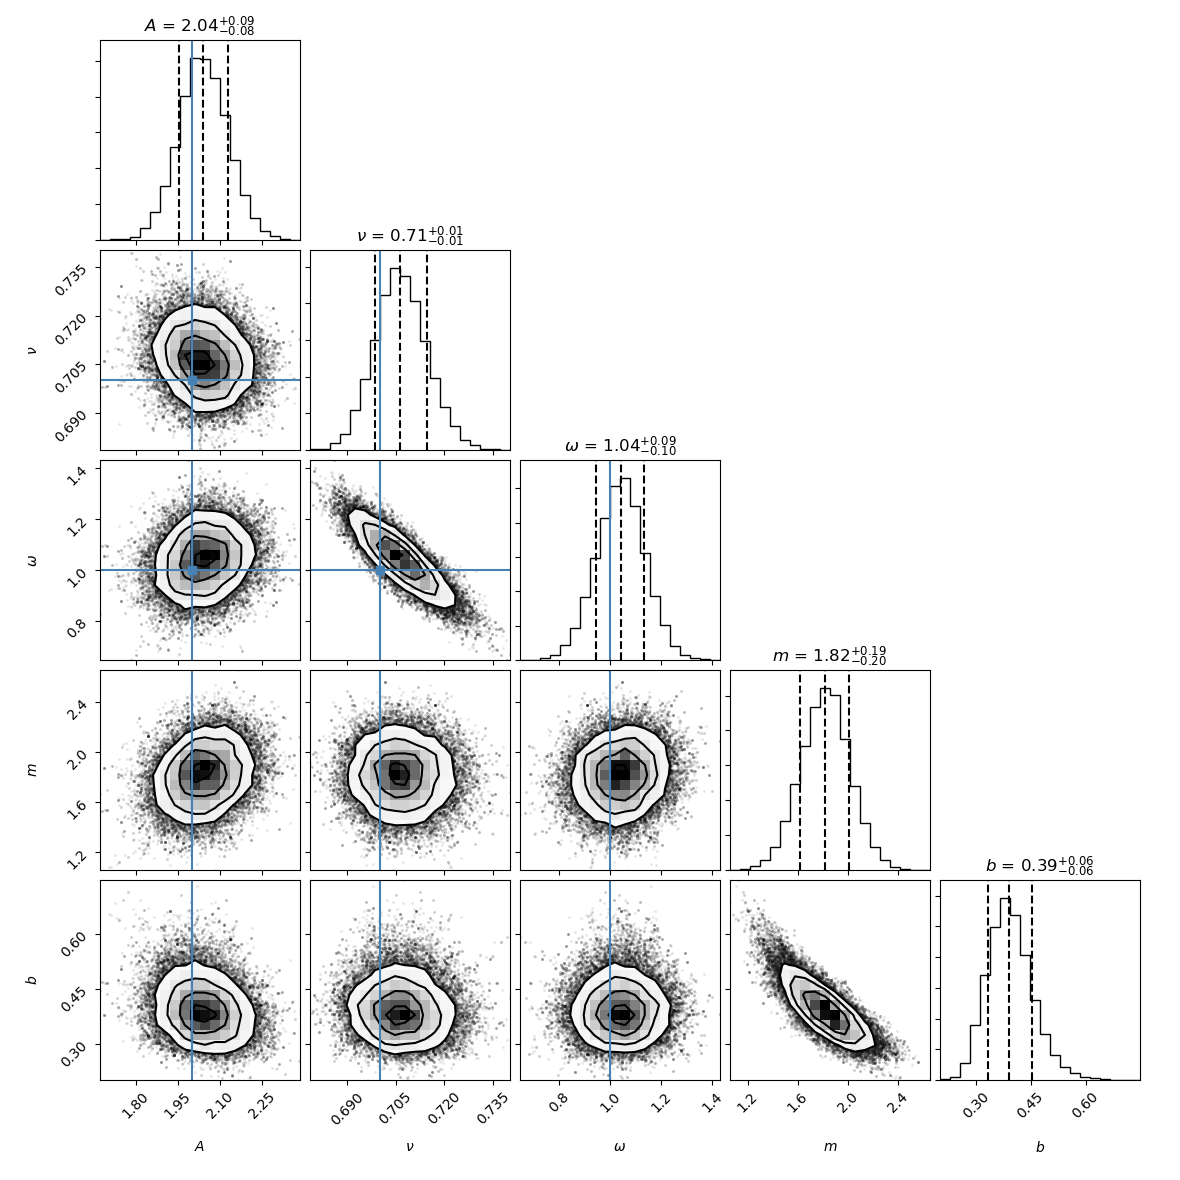
\includegraphics[width=\textwidth]{./Figures/Methods/Fitting_3-MCMC1_XY.png}
        \caption{Jitter correction applied}
    \end{subfigure}	
    \caption[Corner plots of MCMC]
    {Examples of two corner plots showing the successfully recovered planetary orbital parameters (within 10\% of the true values) with MCMC sampling. The blue solid lines indicate the true values of the input orbital parameters. The three dashed lines of each histogram indicate the median and $1\sigma$ on both sides.}
\label{fig:Corner}
\end{figure}    
%-------------

%-------------
\begin{figure}[tbp]	
    \begin{subfigure}[b]{0.49\textwidth}
        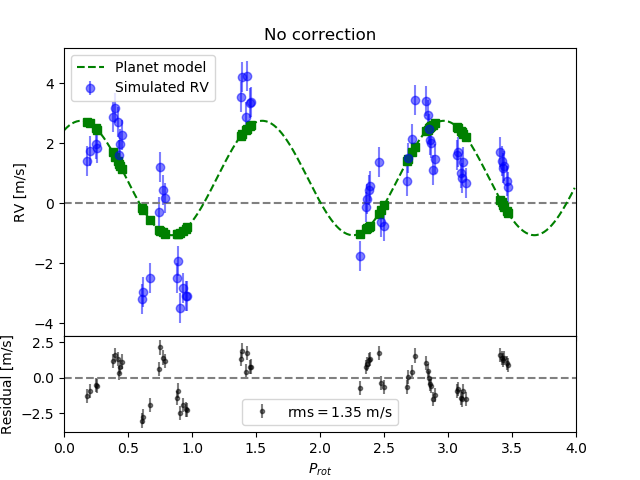
\includegraphics[width=\textwidth]{./Figures/Methods/Fitting_5-Fit2.png}
    \end{subfigure}
	~
    \begin{subfigure}[b]{0.49\textwidth}
        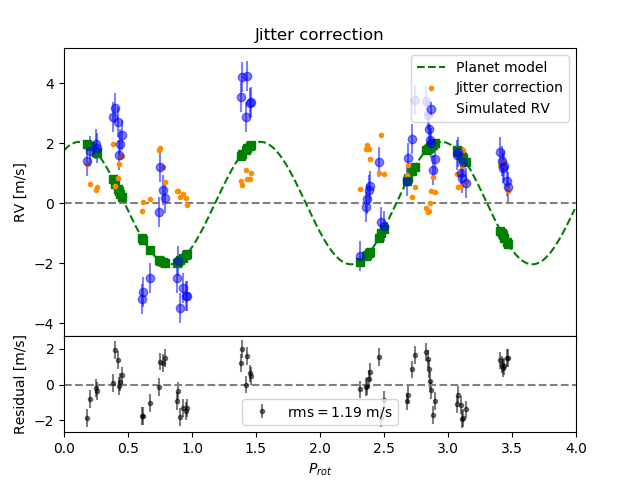
\includegraphics[width=\textwidth]{./Figures/Methods/Fitting_5-Fit1_XY.png}
    \end{subfigure}	
    \caption[Planet recovery ($A = 2$~m/s)]
    {Radial velocity fitting (S/N = 2,000). Theses are two fittings that comes out from the MCMC corner plots in Fig.~\ref{fig:Corner} on the same set of simulated radial velocities. The discrepancy between the simulated radial velocities and the planet model is accounted for by the jitter model, and thus applying the jitter correction reduces the rms of the residual.}
\label{fig:Planet_recovery}
\end{figure}    
%-------------

%-------------
\begin{figure}[tbp]	
    \begin{subfigure}[b]{0.49\textwidth}
        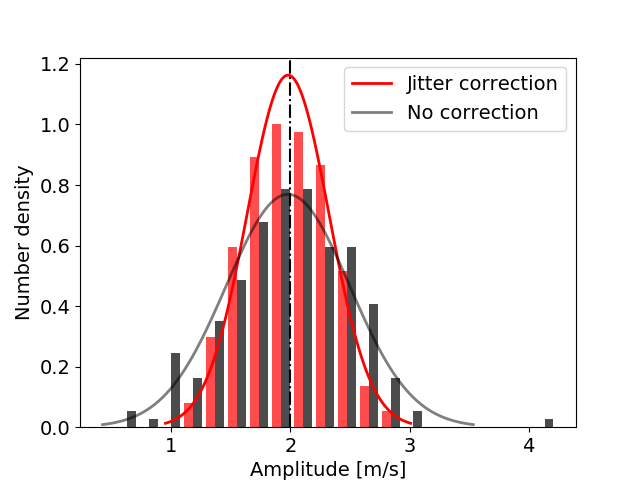
\includegraphics[width=\textwidth]{./Figures/Methods/Histogram_new1.png}
    \end{subfigure}
	~
    \begin{subfigure}[b]{0.49\textwidth}
        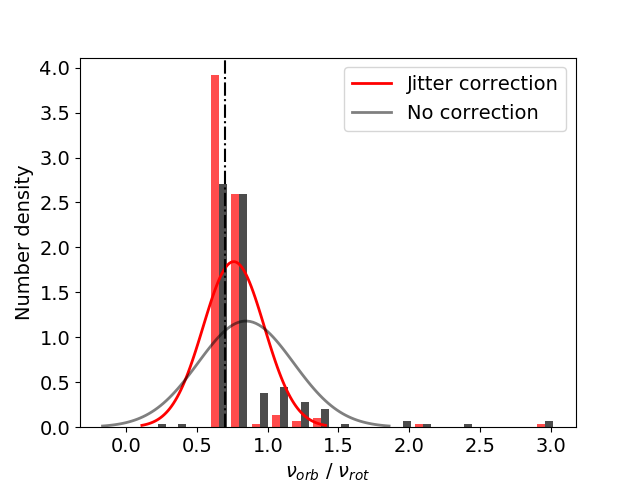
\includegraphics[width=\textwidth]{./Figures/Methods/Histogram_new2.png}
    \end{subfigure}	
    \caption[Histogram of recovered orbital parameters ($A = 2$~m/s)]
    {Histogram of recovered orbital parameters with a Gaussian profile fitted on top. The results from jitter correction are labelled in red (left in the histogram and dark in the Gaussian profile) and that without correction are labelled in grey (right in the histogram and light the Gaussian profile).}
\label{fig:Histogram}
\end{figure}    
%-------------

To quantitatively describe their performances, we calculate the percentage of parameters successfully recovered within 5\% and 10\% of the true values as summarized in Table~\ref{table:a=2}. For example, 15\% of the 200 trails have both the amplitude ($A$) and orbital frequency ($\nu_\text{orb}/\nu_\text{rot}$) successfully recovered within 5\% of the true parameters with jitter correction applied, while only 8\% of them achieve such a precision without jitter correction. 

%-------------
\begin{table}[h!]
\centering
\begin{tabular}{|c|c|c|c|c|}
\hline
\multirow{2}{*}{Percentage} 	& \multicolumn{2}{c|}{5\% limit}  & \multicolumn{2}{c|}{10\% limit}  \\ \cline{2-5} 
                  	& \multicolumn{1}{l|}{$\dagger$} & \multicolumn{1}{l|}{$\ddagger$} & \multicolumn{1}{l|}{$\dagger$} & \multicolumn{1}{l|}{$\ddagger$} \\ \hline
$A$  	 									& 16\% 		& 23\% 			& 32\% 			& 39\%             \\ \hline
$\nu_\text{orb}/\nu_\text{rot}$  			& 40\% 		& 58\%			& 67\%			& 89\%             \\ \hline
both $A$ and $\nu_\text{orb}/\nu_\text{rot}$ & 8\% 		& 15\%			& 23\%			& 37\%             \\ \hline
\end{tabular}
\caption{Proportion of recovered parameters within 5\% and 10\% limit of $A = 2$~m/s and $\nu_\text{orb}/\nu_\text{rot} =0.7$. $\dagger$: no correction; $\ddagger$: jitter correction applied.}
\label{table:a=2}
\end{table}
%-------------
\FloatBarrier

%----------------------------------------------------------------------------------------
\subsection{Planetary signal dominates}

In this case, we set the orbital amplitude roughly 10 times as strong as the jitter, i.e. $A = 20$~m/s (Fig.~\ref{fig:Planet_recovery_a20}). This scenario hardly has impact on obtaining high precision of the orbital parameters of the planets using either approach (Fig.~\ref{fig:Histogram20}), but applying jitter correction slightly improves the performance with overall more precise measurements of the orbital parameters (Table.~\ref{table:a=20}). 

%-------------
\begin{figure}[htbp]	
    \begin{subfigure}[b]{0.49\textwidth}
        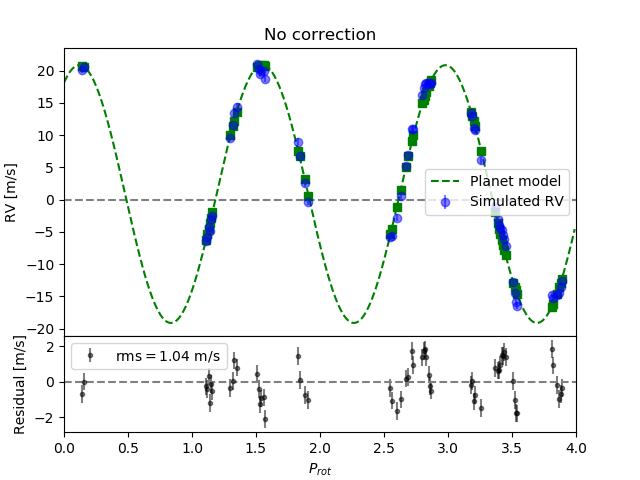
\includegraphics[width=\textwidth]{./Figures/Methods/Fitting_5-Fit2_a20.png}
    \end{subfigure}
	~
    \begin{subfigure}[b]{0.49\textwidth}
        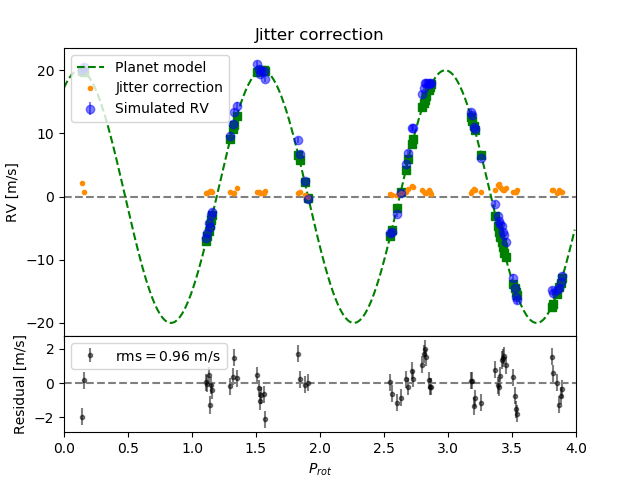
\includegraphics[width=\textwidth]{./Figures/Methods/Fitting_5-Fit1_XYZ_a20.png}
    \end{subfigure}	
    \caption[Planet recovery ($A = 20$~m/s)]
    {Same with Fig.~\ref{fig:Planet_recovery} except the input orbital amplitude of the planet being $A = 20$~m/s.}
\label{fig:Planet_recovery_a20}
\end{figure}    
%-------------

%-------------
\begin{figure}[htbp]	
    \begin{subfigure}[b]{0.49\textwidth}
        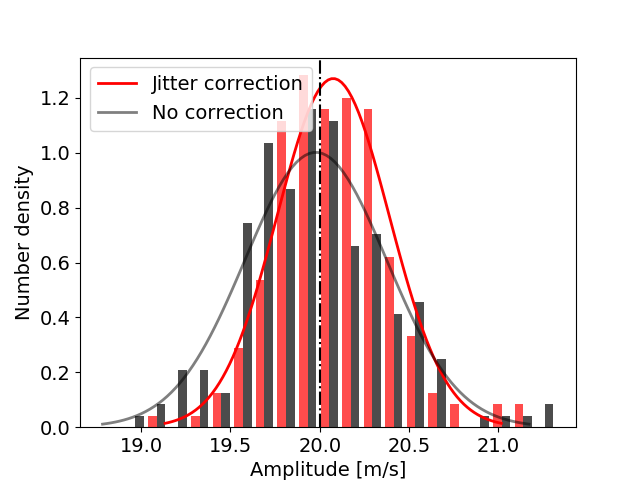
\includegraphics[width=\textwidth]{./Figures/Methods/Histogram_new1_a20.png}
    \end{subfigure}
	~
    \begin{subfigure}[b]{0.49\textwidth}
        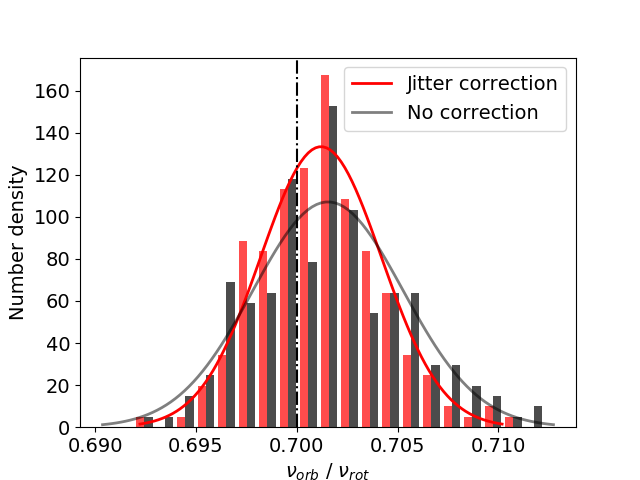
\includegraphics[width=\textwidth]{./Figures/Methods/Histogram_new2_a20.png}
    \end{subfigure}	
    \caption[Histogram of recovered orbital parameters ($A = 20$~m/s)]
    {Same with Fig.~\ref{fig:Histogram} except the input orbital amplitude of the planet being $A = 20$~m/s.}
\label{fig:Histogram20}
\end{figure}    
%-------------

%-------------
\begin{table}[h!]
\centering
\begin{tabular}{|c|c|c|c|c|}
\hline
\multirow{2}{*}{Percentage} 	& \multicolumn{2}{c|}{1\% limit}  & \multicolumn{2}{c|}{5\% limit}  \\ \cline{2-5} 
                  	& \multicolumn{1}{l|}{$\dagger$} & \multicolumn{1}{l|}{$\ddagger$} & \multicolumn{1}{l|}{$\dagger$} & \multicolumn{1}{l|}{$\ddagger$} \\ \hline
$A$  	 									& 41\% 		& 51\% 			& 98\% 			& 99\%             \\ \hline
$\nu_\text{orb}/\nu_\text{rot}$  			& 91\% 		& 97\%			& 100\%			& 100\%             \\ \hline
both $A$ and $\nu_\text{orb}/\nu_\text{rot}$ & 37\% 		& 49\%			& 98\%			& 99\%             \\ \hline
\end{tabular}
\caption{Proportion of recovered parameters within 1\% and 5\% limit of $A = 20$~m/s and $\nu_\text{orb}/\nu_\text{rot} =0.7$. $\dagger$: no correction; $\ddagger$: jitter correction applied.}
\label{table:a=20}
\end{table}
%-------------
\FloatBarrier

%----------------------------------------------------------------------------------------
\subsection{Stellar jitter only}

We set $A=0$~m/s so that the measured the radial velocity only comes from stellar variability. We implement the same approaches as above to see if the applying the jitter correction can return a null planet solution i.e. recovered amplitude smaller than the noise level.

The spot configuration used in Table~\ref{table:spot_configurations} result in the presence of three starspots in turns (Fig.~\ref{fig:rv_recovery_deformed}), mimicking the radial velocities of orbiting exoplanets. This is indeed the case in the histogram of ``recovered" orbital parameters (Fig.~\ref{fig:Histogram_null}) -- three peaks occur at $\nu_\text{orb}/\nu_\text{rot} =$ 1, 2 and 3, with $\nu_\text{orb}/\nu_\text{rot} = 3$ being the most prominent. Applying the jitter correction reduces the amplitude of the candidate in general, making it less likely to be admitted as a true signal than without the use of jitter correction, but still fails to manage to rule out the possibility. 

%-------------
\begin{figure}[htbp]	
    \begin{subfigure}[b]{0.49\textwidth}
        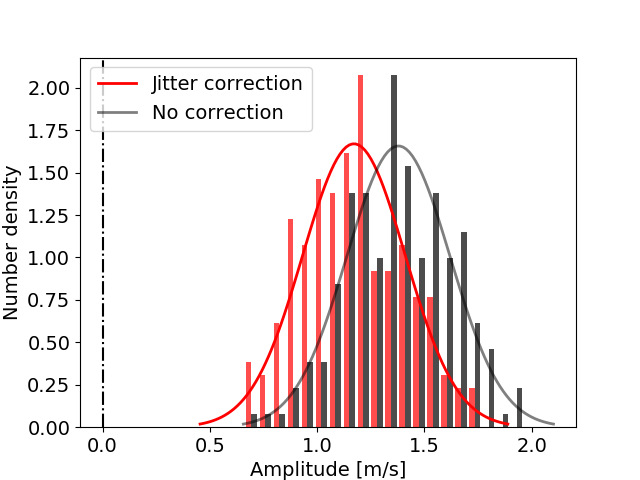
\includegraphics[width=\textwidth]{./Figures/Methods/Histogram_new1_null.png}
    \end{subfigure}
	~
    \begin{subfigure}[b]{0.49\textwidth}
        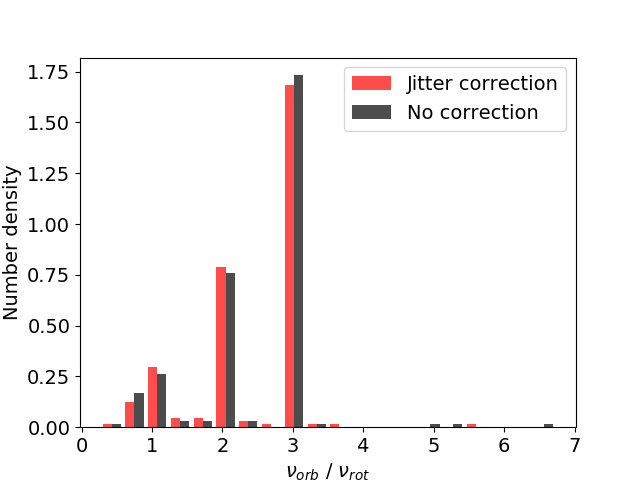
\includegraphics[width=\textwidth]{./Figures/Methods/Histogram_new2_null.png}
    \end{subfigure}	
    \caption[Histogram of recovered orbital parameters of null planets]
    {Histogram of ``recovered" orbital parameters of null planets.}
\label{fig:Histogram_null}
\end{figure}    
%-------------
%\FloatBarrier

%----------------------------------------------------------------------------------------
\subsection{Classification}

We demonstrate the use of the difference in the correlations among $RV_\text{Gaussian}$, $RV_\text{FT,H,L}$ and their combinations as to classify the three scenarios of different relative sizes between the jitter and planetary signals. The discussions are within the captions of Fig.~\ref{fig:correlations}.

%-------------
\begin{figure}[htbp]	
    \begin{subfigure}[b]{1.0\textwidth}
        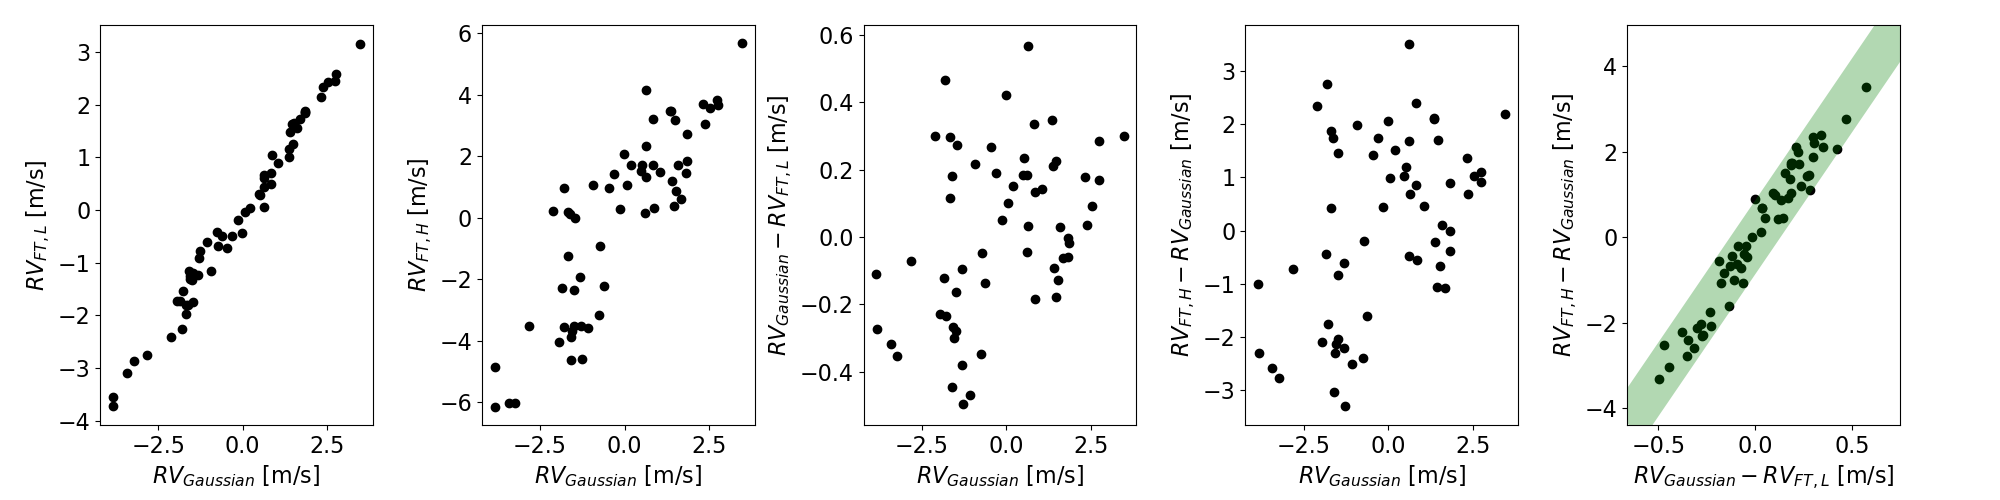
\includegraphics[width=\textwidth]{./Figures/Methods/Correlation_2pj.png}
        \caption{Stellar jitter as strong as planetary signal: featured by (1) a decent correlation between $RV_\text{Gaussian}$ and $RV_\text{FT,L}$ and (2) no correlation between $RV_\text{Gaussian} - RV_\text{FT,H,L}$.}
    \end{subfigure}
	~
    \begin{subfigure}[b]{1.0\textwidth}
        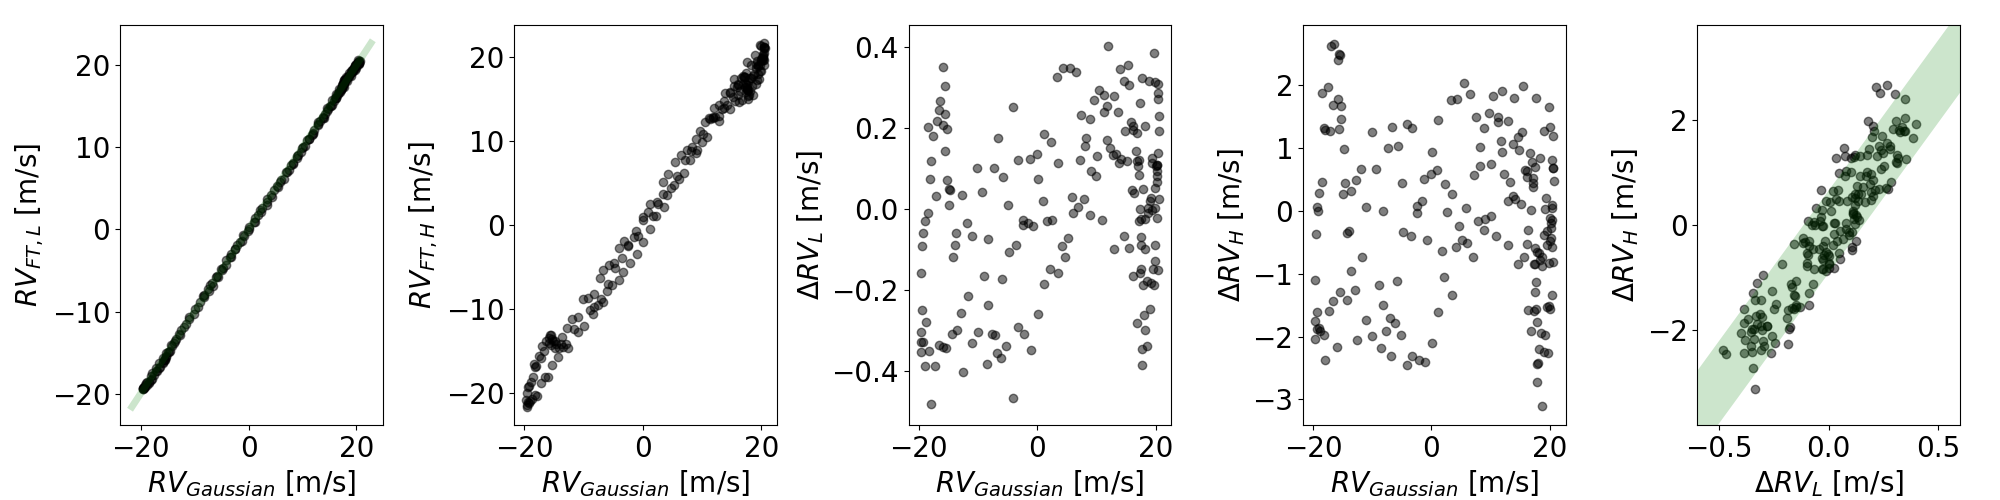
\includegraphics[width=\textwidth]{./Figures/Methods/Correlation_20pj.png}
        \caption{Planetary signal dominating: featured by (1) a tight correlation between $RV_\text{FT,L}$ and $RV_\text{Gaussian}$ and (2) no correlation between $RV_\text{Gaussian} - RV_\text{FT,H,L}$.}
    \end{subfigure}	
	~
    \begin{subfigure}[b]{1.0\textwidth}
        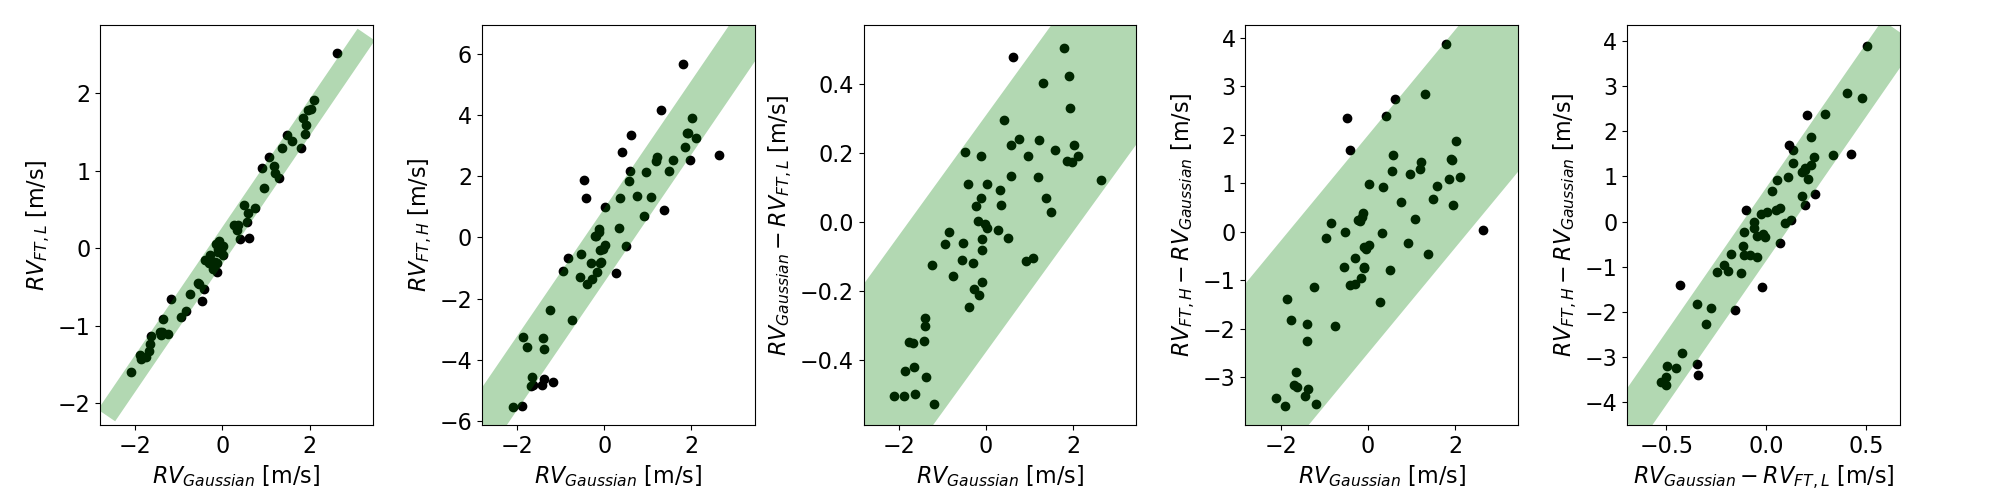
\includegraphics[width=\textwidth]{./Figures/Methods/Correlation_null.png}
        \caption{Jitter only; no planet: featured by linear correlations in all the subplots, on which the Fourier phase spectrum analysis are based.}
    \end{subfigure}	    
	~
    \begin{subfigure}[b]{1.0\textwidth}
        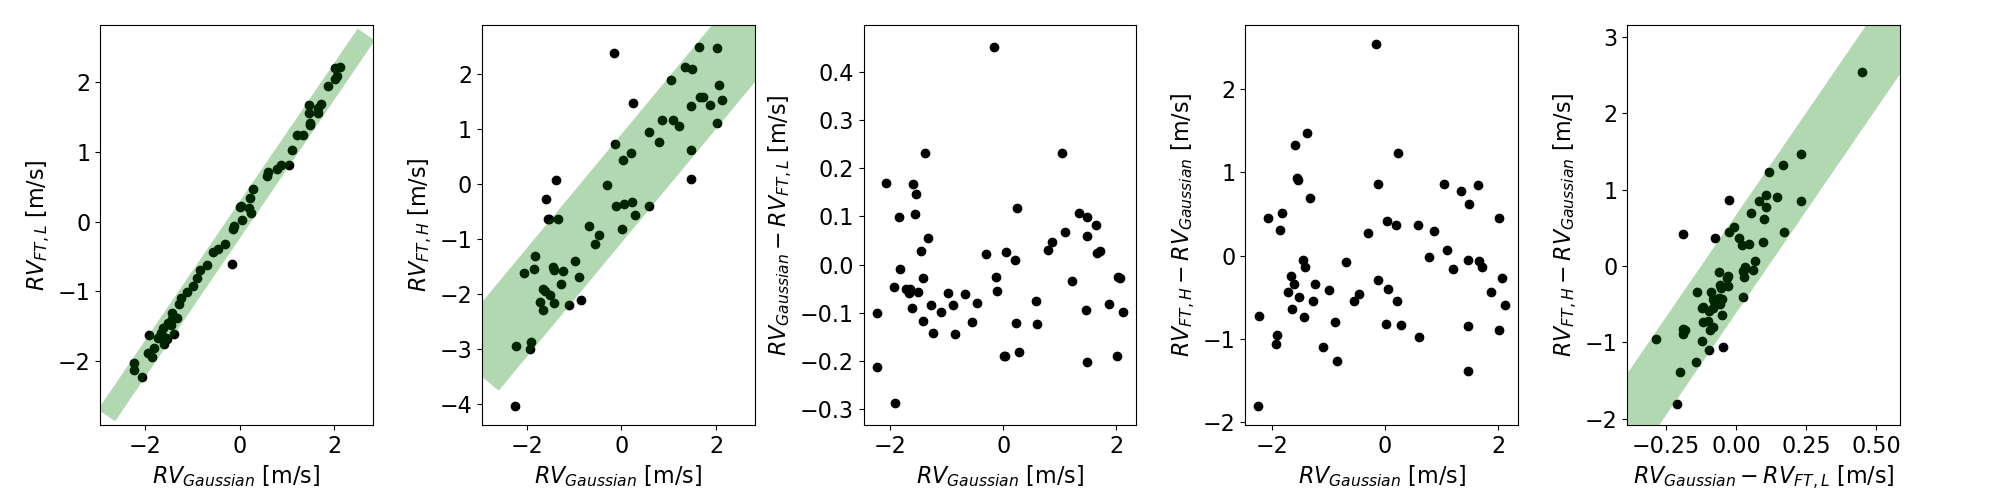
\includegraphics[width=\textwidth]{./Figures/Methods/Correlation_0jitter.png}
        \caption{Planet only; ``no" jitter. No apparent difference from (a) at first sight. This is because the Fourier phase spectrum analysis cannot tell whether the difference between line profiles are due to what we define as stellar jitter or the fluctuation from photon noise, but notice the scales of $RV_\text{FT,H,L}$ in (d) are different from (a), because $RV_\text{FT,H} \approx RV_\text{FT,L} \approx RV_\text{Gaussian}$ without the presence of jitter. }
    \end{subfigure}	    
    \caption[Classification of jitter dominated or planetary signal dominated]        
    {Classification of a system whether it's jitter dominated or planetary signal dominated.}
\label{fig:correlations}
\end{figure}    
%-------------
\FloatBarrier


%----------------------------------------------------------------------------------------
\subsection{Periogodgram combined with the Fourier phase spectrum analysis}

We would use the generalized Lomb-Scargle periodogram \cite{Zechmeister2009} in combination with the Fourier phase spectrum analysis to address the problem of stellar jitter mimicking planetary signals. The idea is to compare the periodogram of the measured radial velocity (i.e. $RV_\text{Gaussian}$) and that of the proto-jitter (i.e. $\mid RV_\text{FT,H/L} - RV_\text{Gaussian} \mid$). Peaks of the periodogram in the former are possible candidates whereas the latter would indicate jitter. 

Fig.~\ref{fig:Periodogram} demonstrates the application of periogodgram together with the Fourier phase spectrum analysis, on the well sampled radial velocities (without sub-sampling) from the two end-to-end simulations in \S\ref{sec:end-to-end}: (1) stellar jitter as strong as planetary signal and (2) stellar jitter only. The S/N of the cross-correlated profile is 2000 and because we used a full range of sampling, no moving average was applied. In Fig.~\ref{fig:Periodogram1} the planetary orbital frequency $\nu_\text{orb}/\nu_\text{rot} = 0.7$ clearly stands out while the other peaks coincide with that of the proto-jitter. It effectively shows, the proto-jitter model generated by the Fourier phase spectrum analysis manages to disentangle jitter from the planetary component of the radial velocities (we recall that the planetary radial velocity was cancelled out to construct the jitter model). In the case of a null planet (Fig.~\ref{fig:Periodogram2}), all the possible candidates where the $RV_\text{Gaussian}$ peaks occur are negated by the same detected periodicity of the jitter. 

%-------------
\begin{figure}[htbp]	
    \begin{subfigure}[b]{0.49\textwidth}
        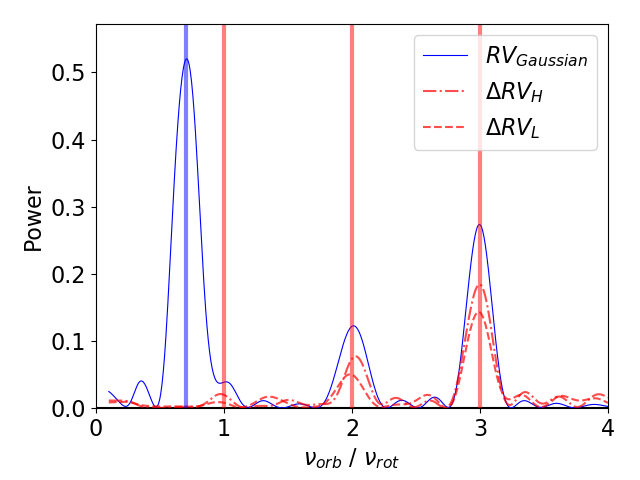
\includegraphics[width=\textwidth]{./Figures/Methods/0-Periodogram_1.png}
        \caption{Stellar jitter as strong as planetary signal}
        \label{fig:Periodogram1}
    \end{subfigure}
	~
    \begin{subfigure}[b]{0.49\textwidth}
        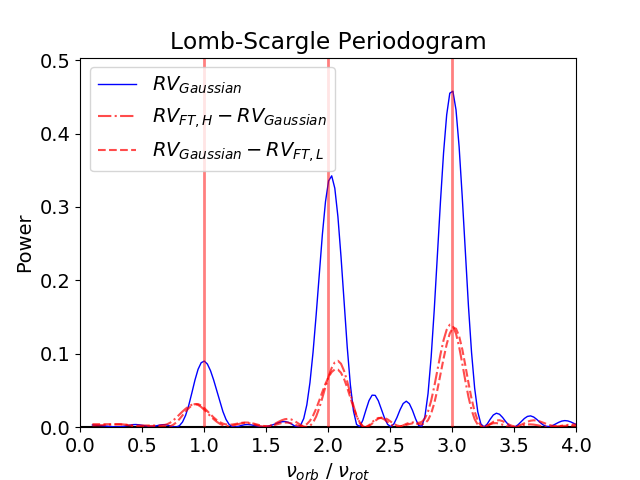
\includegraphics[width=\textwidth]{./Figures/Methods/0-Periodogram_2.png}
        \caption{Stellar jitter only}
        \label{fig:Periodogram2}
    \end{subfigure}	
    \caption[Periodogram combined with the Fourier phase spectrum analysis]
    {Periodogram of $RV_\text{Gaussian}$ and $\mid RV_\text{FT,H/L} - RV_\text{Gaussian} \mid$. The single prominent peak in (a) indicates the orbital frequency (or period) of the injected planet. The true orbital frequency is labelled as the blue vertical line; the suspicious frequencies are labelled in red vertical lines at $\nu_\text{orb}/\nu_\text{rot} =$ 1, 2 and 3.}
\label{fig:Periodogram}
\end{figure}    
%-------------



\pagebreak
%----------------------------------------------------------------------------------------	
%----------------------------------------------------------------------------------------	
\section{Fourier phase spectrum analysis on real observations}
\label{\thesection}
\label{sec:observation}

\subsection{HD189733: Rossiter–McLaughlin effect as jitter}
\label{sec:HD189733}

HD189733 is a well studied binary star system. The main star HD189733~A is known to host a gas giant exoplanet HD189733~b, first detected by transits and followed by Doppler spectroscopy conformation \cite{Bouchy2005ELODIE}. Its Rossiter–McLaughlin effect (Fig.~\ref{fig:rm-effect}), as a change in radial velocities when the planet passes in front of its parent star, was studied by \cite{Cochran2006} and \cite{Triaud2009}. During the eclipse, the planet breaks the observed flux symmetry of the stellar photosphere, resulting in imbalanced redshift and blueshift, producing an asymmetric spectral line profile and apparent radial velocity shifts.

%-------------
\begin{figure}[htbp]
\centering
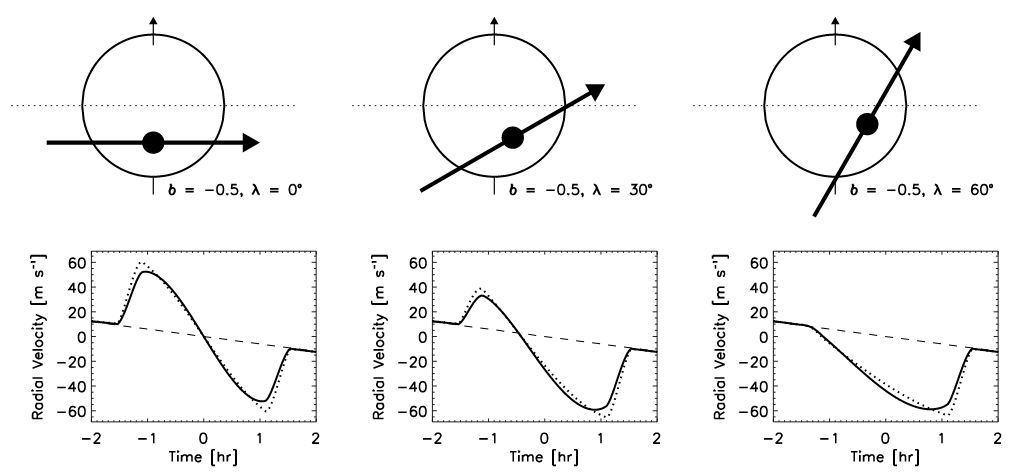
\includegraphics[width = 0.80 \linewidth]
{./Figures/Methods/rmeffect.png}
\caption[Demo: Rossiter–McLaughlin effect]
{Demo: Rossiter–McLaughlin effect (figure taken from \cite{Gaudi2007}). It is an apparent radial velocity change of the parent star due to an eclipsing binary (whether star or planet) in front of the stellar photosphere. It shows in this plot three different star-planet alignments that cause three corresponding different forms of Rossiter–McLaughlin curves. Solid line is the model with limb darkening as opposed to dotted line without limb darkening.}
\label{fig:rm-effect}
\end{figure} 
%-------------

We aim to test if our jitter model generateed by the Fourier phase spectrum analysis can account for the apparent radial velocity shift as a result of Rossiter–McLaughlin effect. We choose this target as a case study for the following reasons: (1) HD189733~b is a confirmed transiting exoplanet, so that we know what to expect from the radial velocity shift during the eclipse. (2) The gas giant exoplanet causes a prominent apparent radial velocity shift while it transits (amplitude up to $\sim 40$~m/s) arising from Rossiter–McLaughlin effect, making it the dominant factor of the radial velocity shift, although the star itself exhibits signs of activity (\cite{Boisse189733}, \cite{Cauley2017}). (3) The system HD189733 has a visual magnitude of $V\sim7.65$ \cite{SIMBAD189733} (or $G=7.41$ from the Gaia archive), dominated by the primary host star HD189733~A, with a relatively high S/N in the HARPS cross-correlation profile, enabling decently good performance of the Fourier phase spectrum analysis in recovering radial velocities.

Here we briefly recap the procedure of obtaining the ``jitter" model by Fourier phase spectrum analysis. Both $RV_\text{Gaussian}$, $RV_\text{FT,H}$ and $RV_\text{FT,L}$) are calculated from the HARPS cross-correlation of the spectral lines. Note that $RV_\text{Gaussian}$, $RV_\text{HARPS}$ and $RV_\text{FT}$ deliver consistent radial velocities, and thus in practice, it barely makes difference to adopt any of them as the radial velocity shift of the line profile. We calculate $\Delta RV = \mid RV_\text{Gaussian} - RV_\text{FT,H/L} \mid$ as the raw proto-jitter (Fig.~\ref{fig:HD189733} bottom left).
We know that during transit, the orbital phase of the planet HD189733~b is zero and thus contributes no radial velocity, however, the inclined trend of the radial velocity curve is attributed to the exoplanet whose orbital period is estimated 11 days \cite{Bouchy2005ELODIE}, as well as the other star HD189733~B in the binary star system of which the orbital period is estimated around 3,200 years \cite{Bakos2006}, both being reasonably long enough as opposed to the time-scale of the planetary transit of hours, therefore a local linear approximation can be applied by fitting a linear trend onto the non-transiting part of the radial velocities as the orbital radial velocities, which is then removed and left with the Rossiter–McLaughlin curve (Fig.~\ref{fig:HD189733} top right). It can be now treated as ``jitter" and modelled by the raw proto-jitter multiplied by a scaling factor (Fig.~\ref{fig:HD189733} right). 

%-------------
\begin{figure}[tbp]
\centering
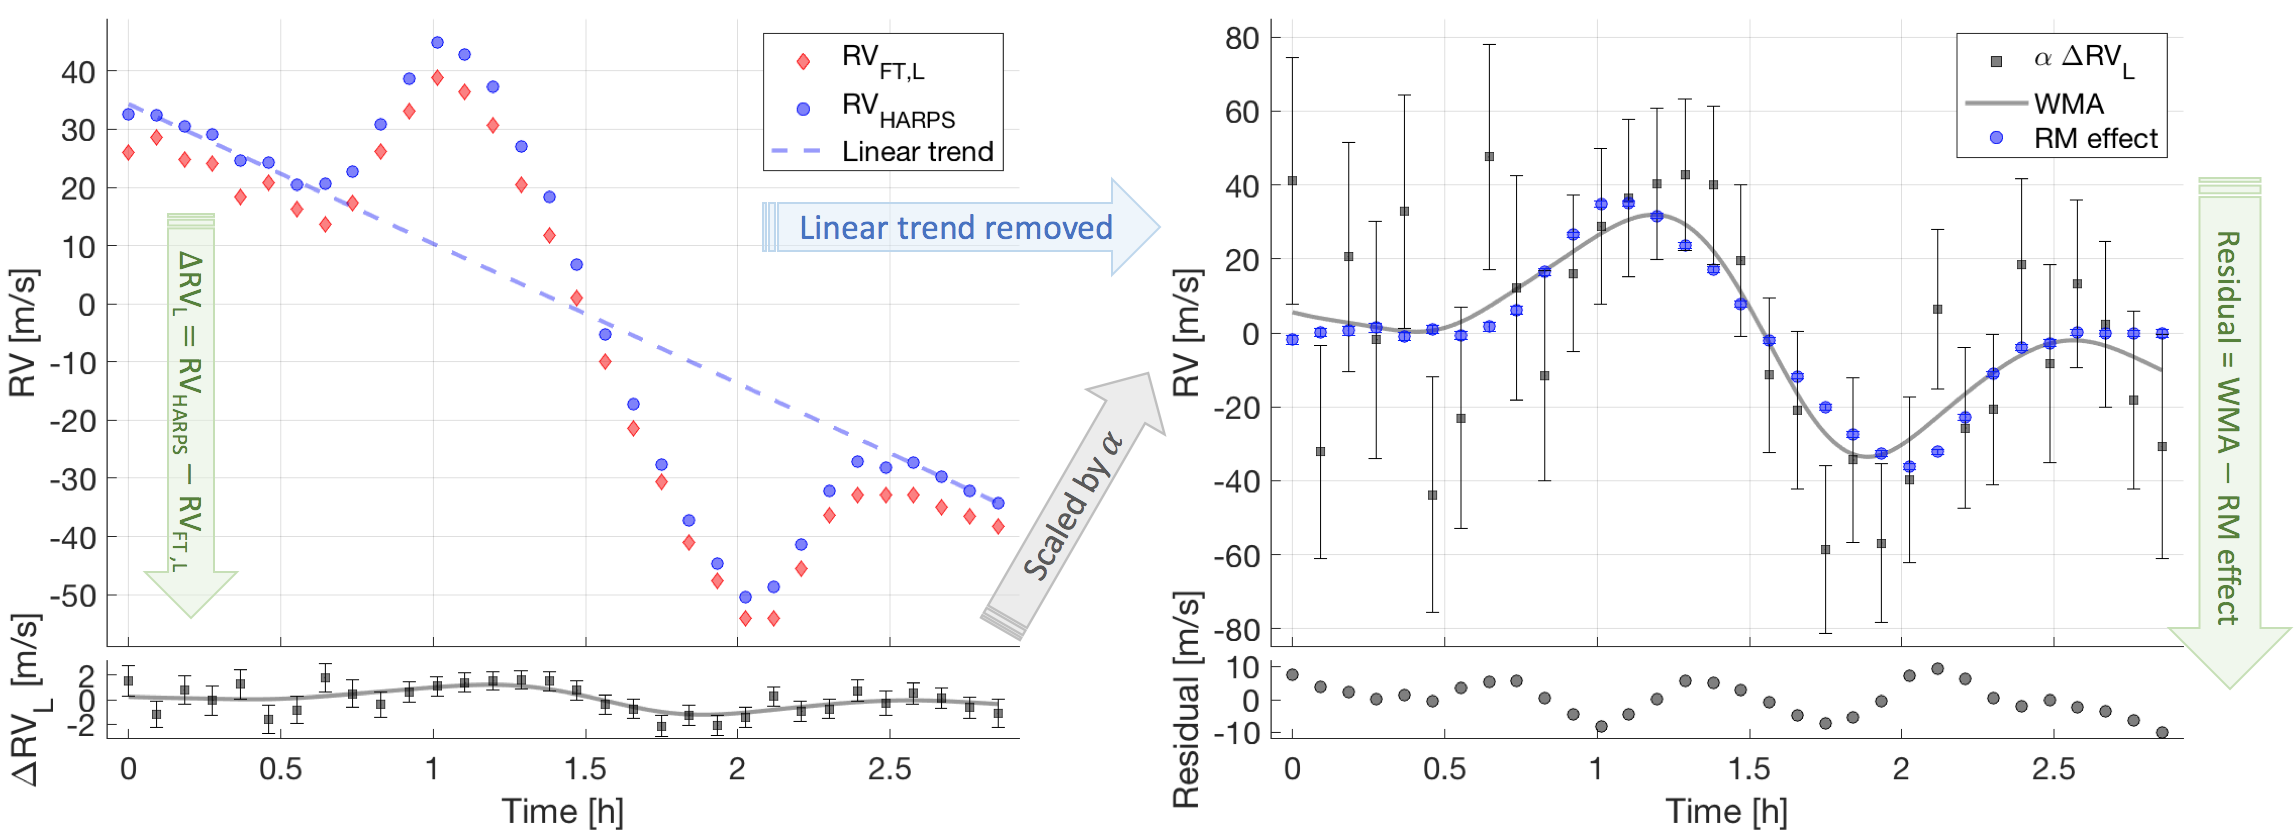
\includegraphics[width = 1.0 \linewidth]
{./Figures/Methods/HD189733.png}
\caption[HD189733: modelling Rossiter–McLaughlin effect as jitter]
		{Flowchart of modelling Rossiter–McLaughlin effect as jitter using Fourier phase spectrum analysis on HD189733. Note that the errorbars related to the radial velocities from Fourier phase spectrum analysis (e.g. the scaled raw jitter in the top right panel) are correct in scale relative to each other (as derived from the photon noise) but not evaluated in the absolute value.}
\label{fig:HD189733}
\end{figure} 
%-------------

For this exercise, the scaled model is smoothed by the weighted moving average with $\tau~\sim0.2$ hour, twice of the spacing of two consecutive observations. Despite mitigating against additional noise brought by the Fourier phase spectrum analysis, it smears the drastic velocity change when the planet ingresses and egresses the stellar disk. Applying a correct Rossiter–McLaughlin curve model is expected to improve the fitting, we still adopt the smoothing approach the way we would normally (intend to) deal with stellar variability induced radial velocities instead, to demonstrate the sufficiently recovered radial velocities as a result of line profile deformation -- a $75\%$ removal of the ``jitter" from $\sim 40$~m/s to $\sim 10$~m/s. 

%The effective length of the smoothing kernel should be carefully chosen. In most cases, it can be chosen roughly the same as the spacing between two consecutive exposures. It can be very useful in mitigating the effect of noise (especially for relatively lower S/N data, to which the Fourier phase spectrum analysis is sensitive, but in this particular Rossiter–McLaughlin effect during the transit, In the future, an adaptive (e.g. S/N dependent) effective length of the smoothing kernel may be implemented to resolve this problem. 
%
%
%When there's no planet or the planetary radial velocity signal is negligible compared with the size of jitter, $RV_\text{FT,L}$ and $RV_\text{FT,H}$ will be proportional to $RV_\text{jitter}$ (Example: \S\ref{sec:HD189733}).

\subsection{$\alpha$ Centauri B (HD128621)}

We have downloaded 2617 $\alpha$ Centauri B spectra from 23/03/2010 to 12/06/2010 from the ESO archive, among which we selected the 2529 cross-correlated line profiles that were constructed with a K5 stellar template; the number of observations that were actually used was then further reduced to 2488 as we took out another 41 observations that presented large radial velocity offsets and visually different cross-correlated line profiles compared with the rest of the profiles. In this way, we can safely believe that the 2488 cross-correlated line profiles differ themselves mainly because of the intrinsic stellar behaviour as well as the presence of orbiting companions, rather than unpredicted causes.

 


\subsection{$\epsilon$ Eridani (HD22049)}

\subsection{$\tau$ Ceti (HD10700)}

%HD\,49933 is an F2 main sequence star with an apparent magnitude of $m_V=5.8$ (\cite{Malaroda1975}), 



\FloatBarrier

%----------------------------------------------------------------------------------------
%\clearpage
\section{References}
\label{\thesection}
\vspace{-1.5cm}
\setstretch{1.0}
\bibliographystyle{unsrt}
\bibliography{Bibliography}
\setstretch{1.3}
